\documentclass[12pt,titlepage]{article}
\usepackage[table]{xcolor}
\usepackage{longtable}
\usepackage[utf8]{inputenc}
%Language of Document Elements like Figure or Table
\usepackage[english]{babel}
\usepackage[bookmarks]{hyperref}
\usepackage{pdfpages}
\usepackage{graphicx}
\usepackage{float}
\usepackage{colortbl,array}
\usepackage[justification=centering]{caption}
\usepackage{enumitem}
\usepackage{chngcntr}
\usepackage{lscape}
\usepackage{fancyhdr}
\usepackage{listings}
\usepackage{hyperref}
\usepackage{nameref}
\usepackage{tabularx}
\usepackage[a4paper,width=160mm,top=25mm,bottom=25mm]{geometry}
\usepackage[ngerman]{translator}
\usepackage{acronym}
\usepackage{listings}
\usepackage{makecell}
\usepackage{rotating}


\definecolor{warningbackground}{RGB}{252,226,158}

\newcommand{\alertwarningbox}[1]{
	\begin{tabularx}{\linewidth}{
			>{\columncolor{warningbackground}}c
			>{\columncolor{warningbackground}}X}
		\raisebox{\dimexpr2\baselineskip-\height} &
		\raisebox{\tabcolsep}{\strut}#1\raisebox{-\tabcolsep}{\strut}
	\end{tabularx}
}

%Syntax-highlighting]
%\usepackage{minted}
%\usemintedstyle{vs}

%Each Section in a new Page
\let\oldsection\section
\renewcommand\section{\clearpage\oldsection}

%Fix for to long Roman letters
\makeatletter 
\renewcommand{\@pnumwidth}{5em} 
\makeatother

%Set space around and between lists
\setlist[enumerate]{noitemsep, topsep=0cm}
\setlist[itemize]{noitemsep, topsep=0cm}

%Figure/Table Numbering style "Section Number.figure counter
\renewcommand{\thefigure}{\arabic{section}.\arabic{figure}}
\renewcommand{\thetable}{\arabic{section}.\arabic{table}}

%Reset figure/table counter after section change
\counterwithin{figure}{section}
\counterwithin{table}{section}

\hypersetup{
	colorlinks,
	linkcolor={black},
	citecolor={black},
	urlcolor={black}
}

\colorlet{punct}{red!60!black}
\definecolor{background}{HTML}{EEEEEE}
\definecolor{delim}{RGB}{20,105,176}
\colorlet{numb}{magenta!60!black}

\newcommand{\todonl}[1]{\newline\textcolor{red}{TODO: #1}\PackageWarning{TODO:}{#1!}}
\newcommand{\todo}[1]{\textcolor{red}{TODO: #1}\PackageWarning{TODO:}{#1!}}

%Set Paragraph indent to null
\setlength{\parindent}{0pt}
% Smaler Table Space
\renewcommand{\arraystretch}{1.5}

% renamig of section to Abschnitt \autoref
\addto\extrasenglish{%
	\def\sectionautorefname{Abschnitt}%
}

% renamig of subsubsection to Abschnitt \autoref
\addto\extrasenglish{%
	\def\subsubsectionautorefname{Abschnitt}%
}

% renamig of subsection to Abschnitt \autoref
\addto\extrasenglish{%
	\def\subsectionautorefname{Abschnitt}%
}
%rename Figure zu Abbildung
\addto\captionsenglish{\renewcommand{\figurename}{Abbildung}}

%rename Tabe zu Tabelle
\addto\captionsenglish{\renewcommand{\tablename}{Tabelle}}


% Befehle für die Tabellenerstellung der Testcases
\newcommand{\testpttb}[3]{
%	\begin{landscape}
		\subsection{#1}
		#2
		\rowcolors{2}{gray!25}{white}
		\begin{longtable}{| m{0.5cm} | m{9cm} | m{6cm} | m{6cm} | m{1.5cm} |}
			\caption{#1} %\label{tab:#1}
			\endlastfoot
			\hline
			\textbf{Nr} & \textbf{Beschreibung} & \textbf{Erwartetes Ergebnis} & \textbf{Tatsächliches Ergebnis} & \textbf{Status}
			\\
			\hline
			#3
			\hline 
		\end{longtable}
%	\end{landscape}
}

\newcommand{\testptrow}[5]{
	#1 & #2 & #3 & #4 & #5 \\
}

\title{Krisenresistente Software Defined Netzwerke}
\author{Sandro Kaspar, Jessica Kalberer}
\date{17.09.2018}

\pagestyle{fancy}
\lhead{Krisenresistente Software Defined Netzwerke}
\begin{document}
\pagenumbering{Roman}



\includepdf{pdfincludes/titlepage}

\newpage
%new Title for tableofcontent
\renewcommand{\contentsname}{Inhaltsverzeichnis}
\tableofcontents
\newpage
\pagenumbering{arabic}

\section{Aufgabenstellung}
Dies ist die initiale Aufgabenstellung, welche zu Beginn der Bachelorarbeit vorlag. 

\subsection{Erster Teil ($\sim$10\%): Phase Analyse}
Ziel: Sämtliche Analyse der SDA Lösung und Identifizierung der kritischen Elemente der Verfügbarkeit (LISP Database, Radius, SGT Access-list, etc.) und der Network Services (NTP, DNS, Lizenzen, etc.)
\begin{itemize}
	\item Die Clients werden am Netz mit dot1x authentifiziert und mit Wired Access verbunden (Wireless Access ist nicht Teil der Bachelorarbeit)
\end{itemize}


\subsection{Zweiter Teil ($\sim$45\%): Phase Absicherung}
Ziel: Erstellung von Technische Design und Ansätze um die SDA Lösung Krisenresistenter zu machen.
\begin{itemize}
	\item Die Arbeiten umfassen:
	\begin{itemize}
		\item Analyse und Gegenüberstellung der mögliche Optionen für die Verbindungen von zwei SDA Fabric (VRF-Lite, Transit Fabric, etc.)
		\item Empfehlungen für das Deployment eines krisensicheren SDA
		\item Aufbau eines Pilots mit mindestens zwei Standorten
		\item Durchführung der definierten Vorgaben im Pilot
	\end{itemize}
	\item Ein ECNS 5000 wird zur Verfügung gestellt und kann in der krisensicheren Lösung integriert sein.
\end{itemize}


\subsection{Dritter Teil ($\sim$45\%): Phase Abstrahierung}
Ziel: Entwicklung eines Operations Orchestrators für 2-{\tiny }3 Use Cases. 
\begin{itemize}
	\item Die Use cases werden von Betreuern und Industiepartner festgelegt.
	\item Der Operations Orchestrator wird bestimmte Operations Tätigkeiten vereinfachen und wird mit DNA Center, ISE und dem Fusion Router interagieren. (Wenn zwei VRFs zusammen kommunizieren werden die Fabric und der Fusion Router gleichzeitig konfiguriert)
	\item Idealerweise gibt es ein Web Interfaces für Demozweck.
\end{itemize}

Notwendige Kenntnisse: Routing\&Switching, VXLAN Overlays, Network Services, objektorientierte Programmierung (Python bevorzugt)



\section{Abstract} 

\subsection{Aufgabenstellung} 
Die Aufgabe dieser Bachelorarbeit war es, eine verteilte, krisenresistente Software-Defined Access (SDA) Lösung für die Führungsunterstützungsbasis der Armee (FUB) zu erstellen. Dies basierend auf dem DNA Center von Cisco, welches bereits in einer Studienarbeit in Betrieb genommen wurde. In einem ersten Schritt wurden die kritischen Komponenten der Lösung identifiziert und Ansätze entwickelt, wie diese Komponenten abgesichert werden können. Im darauffolgenden Schritt wurden diese Ansätze konkretisiert und umgesetzt. Der dritte Teil der Aufgabe war, ein Orchestrierungstool zu entwickeln, welches die gängigsten Operations Tasks vereinfacht und teilweise automatisiert. Folgende Use Cases soll die Anwendung abdecken:
\begin{itemize}
	\item Netzwerke erstellen und verwalten
	\begin{itemize}
		\item Netzwerke im DNA Center anlegen
		\item Konfiguration der Fusion Router
		\item Access Policies zwischen den Netzwerken konfigurieren
	\end{itemize}
	\item Management der virtuellen Maschinen
	\item Anzeigen aller Konfigurationen und der dazugehörigen History
\end{itemize}


\subsection{Vorgehen}
In dieser Bachelorarbeit wurden grundlegende Ansätze zum Betrieb einer SDA Lösung erarbeitet, die in Zukunft weiterentwickelt werden können. Zu Beginn wurde das Lab, welches in der Studienarbeit erstellt wurde analysiert und die kritischen Komponenten, die für den Betrieb der Umgebung nötig sind, identifiziert. Zudem wurden Ideen entwickelt, wie diese kritischen Komponenten abgesichert und redundant betrieben werden können, sodass der Betrieb auch bei Ausfall von Komponenten oder Verbindungen gewährleistet ist. Ebenfalls wurde die Architektur der Umgebung analysiert und verbessert, sodass die Anforderungen an die Verfügbarkeit erfüllt sind. In einem nächsten Schritt wurden die zuvor erarbeiteten Ideen in der Testumgebung praktisch umgesetzt und getestet. Für viele Services, die in der verteilten Umgebung an allen Standorten verfügbar sein müssen, wurde eine Virtualisierungsplattform von Cisco verwendet. Im dritten Teil der Arbeit wurde ein Orchestrierungstool entwickelt. Mit Hilfe von diesem kann ein Operator die gängigsten Aufgaben über ein Web-Interface ausführen. Das Tool automatisiert zudem Arbeitsschritte, die im DNA Center noch nicht abgedeckt sind und manuell ausgeführt werden müssten. 

\subsection{Fazit}
Es kann gesagt werden, dass die zentrale Struktur einer SDA Lösung die Sicherstellung der Verfügbarkeit in einer verteilten Umgebung erschwert. Die kritischen Komponenten, die in der Analyse definiert wurden, konnten dennoch zum grössten Teil erfolgreich abgesichert werden. Allerdings ermöglichen die zentralen Controller dieser Struktur ein programmatisches und automatisiertes Management der Infrastruktur über APIs. Nicht nur aus diesem Grund ist das Software-Defined Netzwerk (SDN) definitiv das Netzwerk der Zukunft. 


\section{Danksagung}

Die Arbeit an diesem Projekt währe ohne die Hilfe die wir von verschiedenen Personen erhalten haben, nicht möglich gewesen. Dank ihrer Beiträge war es möglich, den Projektstand zu erreichen, den diese Arbeit jetzt hat.

\begin{itemize}
	\item Prof. Laurent Metzger für seine ausgezeichnete Betreuung und vielen hilfreichen Inputs
	\item Urs Baumann für seine wertvollen Beiträge und die ausgezeichnete Co-Betreuung
	\item Patrick Mosimann für die zeitnahe Beantwortung unserer vielen Fragen und Unterstützung 
	\item Laurent Billas für die gute und konstruktive Zusammenarbeit
	\item Serge Pidoux für die gute und konstruktive Zusammenarbeit
\end{itemize}

Natürlich möchten wir uns auch bei den Menschen bedanken, die nicht namentlich erwähnt werden, die aber während der ganzen Bachelorarbeit mentale Unterstützung leisten, immer ein offenes Ohr für uns haben und uns auf unserem Weg stets unterstützen, wie zum Beispiel unsere Familien.
\section{Management Summary}

\subsection{Ausgangslage}
Diese Bachelorarbeit ist eine Folgearbeit der Studienarbeit \textit{Software-Defined Netzwerk im Campus Bereich} \cite{studienarbeit}. Ziel der Studienarbeit war die Evaluation des Cisco Digital Network Architecture (DNA) Center, der Software-Defined Network (SDN) Lösung von Cisco, für die Führungsunterstützungsbasis (FUB) der Schweizer Armee. In der Studienarbeit wurden mit den vorhandenen Geräten zwei Standorte geplant. Auf Grund von aufgetretenen Problemen und Bugs wurde entschieden, sich nur auf einen Standort mit mehreren Devices und zwei Gebäuden zu konzentrieren. Für diesen Standort wurde eine Fabric mit zwei Sites erstellt und diverse Policies implementiert. Somit konnten die vorgegebenen Use Cases, wie zum Beispiel die Definition von Benutzerprofilen, Benutzermobilität oder Reporting der Netzwerkaktivitäten umgesetzt und getestet werden.

\subsection{Vorgehen}
Nun soll in dieser Bachelorarbeit in einem ersten Schritt die SDN Lösung analysiert und sämtliche kritischen Elemente identifiziert werden. Zudem wurden Ideen entwickelt, wie diese kritischen Komponenten abgesichert und redundant betrieben werden können, sodass der Betrieb auch bei Ausfall von Komponenten oder Verbindungen jederzeit ge\-währ\-leis\-tet bleibt. In einem zweiten Schritt werden die kritischen Elemente wenn möglich abgesichert und eine Empfehlung für das Deployment eines krisensicheren SDN erarbeitet. Neu hinzu kam auch die Virtualisierungsplattform ENCS 5400, welche verwendet wurde, um einen autonomen Standort zu simulieren. Zum Abschluss erfolgt das Abstrahieren einzelner Elemente, welche im Verlauf der Bachelorarbeit noch in Use Cases definiert wurden, aus dem DNA Center in ein eigen entwickeltes Orchestrierungstool. 

\subsection{Ergebnisse}
Als Ergebnis dieser Bachelorarbeit steht ein möglichst krisensicherer Prototyp zur Ver\-fü\-gung. Der Prototyp besteht aus den Cisco Komponenten sowie Eigenentwicklungen, die zu\-sätz\-liche Features implementieren. Zudem steht eine Dokumentation des Systems zur Verfügung, welche eine Analyse der kritischen Komponenten, eine Empfehlung für das Deployment eines krisensicheren SDN, sowie eine Dokumentation über das eigen entwickelte Or\-ches\-t\-rie\-rungstool beinhaltet. Über das eigen entwickelte Orchestrierungstool können ausserdem einzelne Standard-Aufgaben unabhängig vom DNA Center ausgeführt werden. Dies soll zum einen Aufgaben vereinfachen, in dem diese beispielsweise mit einem Wizard durchlaufen werden können. 
 
\subsection{Ausblick}
Die Resultate dieser Arbeit können dazu dienen, eine möglichst krisensichere SDA Lösung in einer produktiven Umgebung in Betrieb zu nehmen. Zudem kann der Prototyp um zusätzliche Funktionen erweitert, an bestehende oder neue Systeme angebunden oder mit alternativen Lösungen verglichen werden. Durch das eigen entwickelte Orchestrierungstool wurden die Möglichkeiten welche das DNA Center zur Zeit durch seine API bietet evaluiert. Die API von Cisco bietet schon viele Möglichkeiten, jedoch lassen die API Dokumentationen sehr zu wünschen übrig, da viele Funktionalitäten veraltet oder gar nicht dokumentiert sind. Dies wird mit hoher Wahrscheinlichkeit aber in neuen Releases des DNA Centers behoben.

%\section{Problembeschreibung}


\section{Einführung}

Wie schon erwähnt ist diese Bachelorarbeit eine Folgearbeit der Studienarbeit Software-Defined Netzwerk im Campus Bereich \cite{studienarbeit}, was bedeutet das in dieser Arbeit nicht mehr auf die grundlegenden Technologien eingegangen wird. Es werden jedoch Technologien, welche für das krisenresistente Netzwerk besonders relevant sind, detaillierter analysiert und beschrieben. 

\subsection{Erkenntnisse aus der Studienarbeit}

In der Studienarbeit hat sich klar herauskristallisiert, dass bei einer so grossen Organisation wie der FUB ein besonderes Augenmerk auf die Skalierbarkeit gelegt werden muss. Auf Grund der aufgetretenen Probleme und Bugs, konnten diese Anforderungen jedoch nur kurz angeschnitten werden. Im Verlauf der Studienarbeit wurde eine laufende Fabric mit der höchsten Priorität definiert. Darauf folgend konnten die vom Industriepartner definierten Use Cases praktisch und wenn nicht anders möglich theoretisch abgedeckt werden. Die Use Cases lauteten folgendermaßen \cite{studienarbeit}:

\begin{itemize}
	\item Definition von Benutzerprofilen
	\item Benutzermobilität
	\item Reporting der Netzwerkaktivitäten
	\item Degradation der Infrastruktur
	\item Backup und Restore
	\item Anbindung an externe Systeme, wie ISE und Infoblox
\end{itemize}


Wie bei neuerer Software üblich, waren auch in DNA Center noch verhältnismässig viele
Bugs vorhanden. Die Bugs wurden in der Studienarbeit dokumentiert und jeweils an die Cisco
Experten weitergeleitet. Teilweise konnten die Bugs durch neue Releases schon behoben werden, wiederum andere sind noch ausstehend. 


\subsection{Krisenresistentes Software Defined Netzwerk}
Nun soll in dieser Bachelorarbeit ein krisenresistentes Netzwerk erstellt werden, welches mit Hilfe des DNA Centers und Technologien wie VXLAN und LISP einsetzt, welche in der Studienarbeit genauer dokumentiert wurden \cite{studienarbeit}. In der Bachelorarbeit wird zum einen ein möglichst krisenresistentes Netzwerk erstellt und für dies eine Empfehlung für das Deployment vorgestellt. Zum anderen sollen die API des DNA Centers genauer untersucht und in einem eigen entwickelten Orchestrierungstool verwendet werden. In der Studienarbeit waren bis dato nur wenige Informationen zu der API verfügbar, welche nun mit dem Release 1.2.5 aber relativ gut abgedeckt sein sollten. In der Analyse der ganzen SDA Lösung sollen nun auch die Skalierbarkeit genauer untersucht werden, ob dies mit den aktuellen Empfehlungen von Cisco, für so eine grosse Organisation wie der FUB überhaupt in umgesetzt werden kann. Mit einem ECNS 5400 soll zudem ein autonomer Standort mit den nötigen Diensten wie Radius, DHCP, DNS und NTP simuliert werden können.






\section{Analyse}
Nachfolgend werden alle kritischen Elemente der SDA Lösung analysiert. Dazu gehören beispielsweise Dienste, wie die LISP Datenbank, Radius, SGT Access List. und 

Das Ziel ist die komplette Analyse der SDA Lösung und die Identifizierung der kritischen Elemente der Verfügbarkeit (LISP Database, Radius, SGT Access-list etc.) und der Network Services (NTP, DNS, Lizenzen etc.).

\subsection{SDA Architektur und Design}
Unsere Architektur der Lab Umgebung, welche in der Studienarbeit erarbeitet und nun in der Bachelorarbeit noch erweitert wurde, sieht zur Zeit wie folgend aus:

\begin{figure}[H]
	\centering
	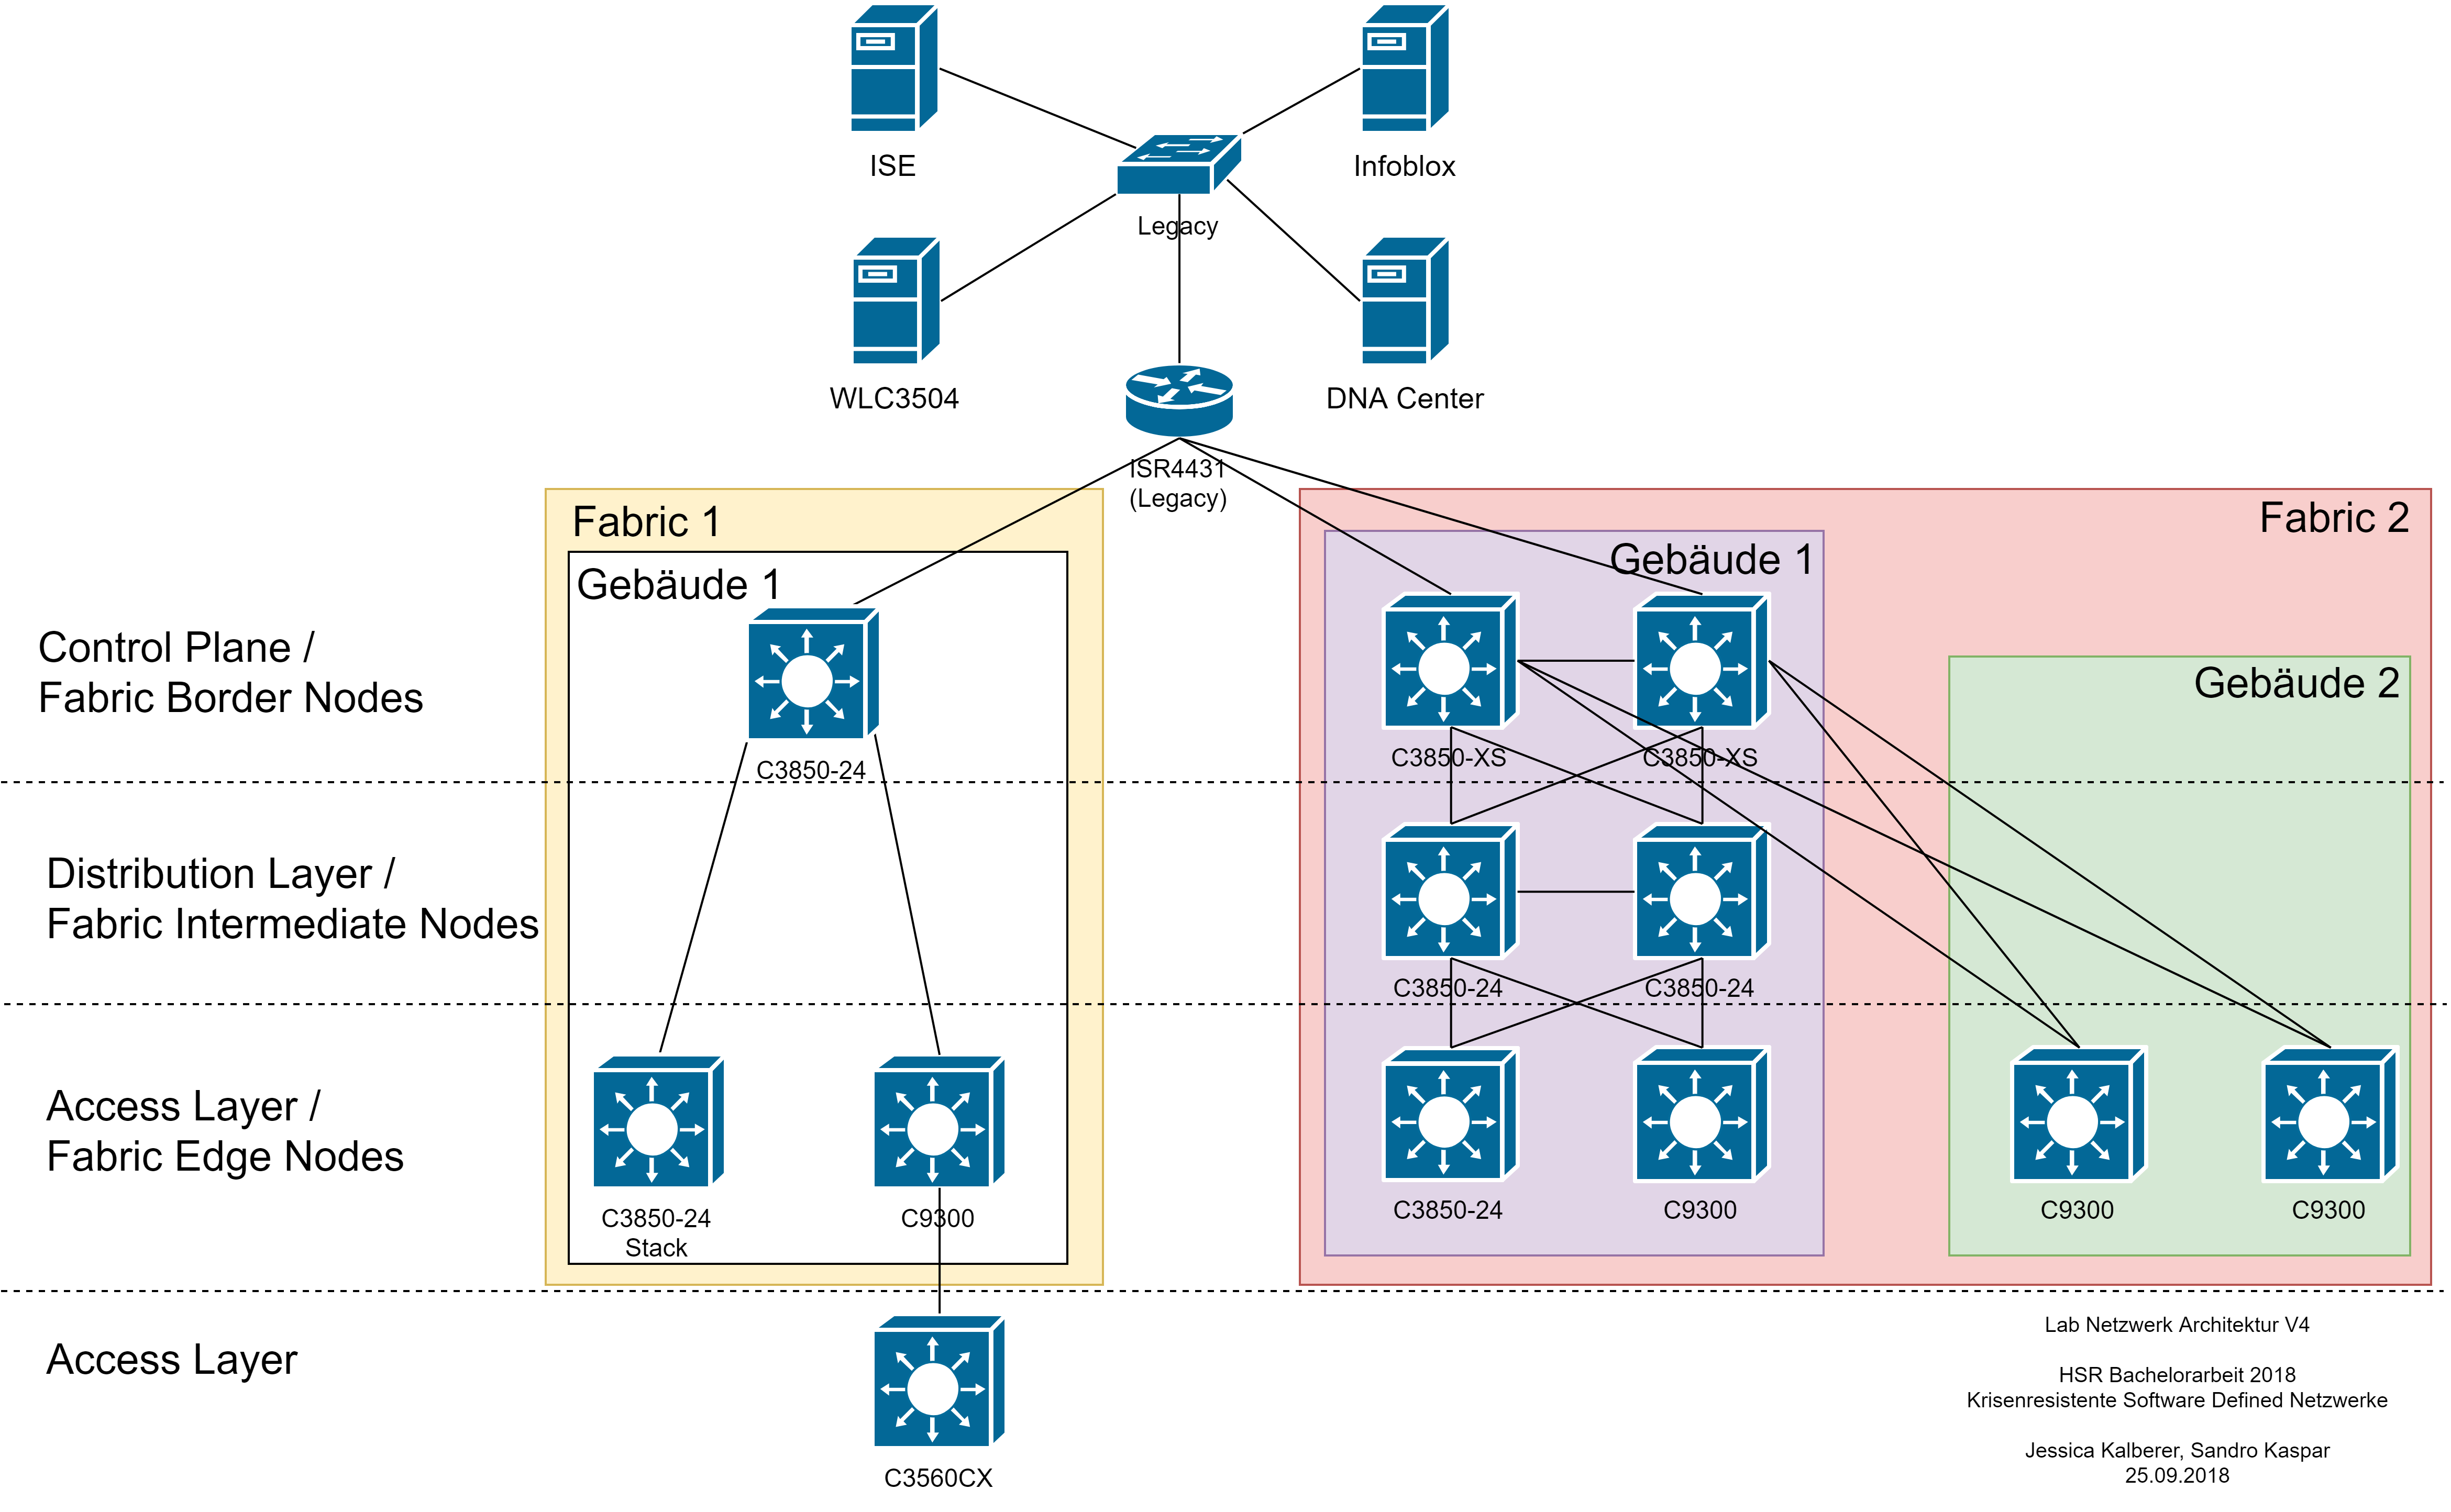
\includegraphics[width=1\linewidth]{img/Architecture/LabNetworkArchitecture-25-09}
	\caption{Architektur}
	\label{fig:Architektur}
\end{figure}

Die Analyse wird auf dieser Architektur aufbauen und die von der FUB gegebenen Grössenordnung berücksichtigen.

Nachfolgend werden die aktuell von Cisco empfohlenen Design Entscheidungen, Grössenüberlegungen, sowie die Skalierungen gezeigt. Aktuelle und ausführliche Informationen hierzu, können direkt im SDA Design Guide von Cisco \cite{sda-designguide} eingesehen werden. 

\subsubsection{Entscheidungen}
Die Design Entscheidungen beruhen auf den aktuellen Empfehlungen von Cisco, welche sich laufend Ändern können.

\begin{figure}[H]
	\centering
	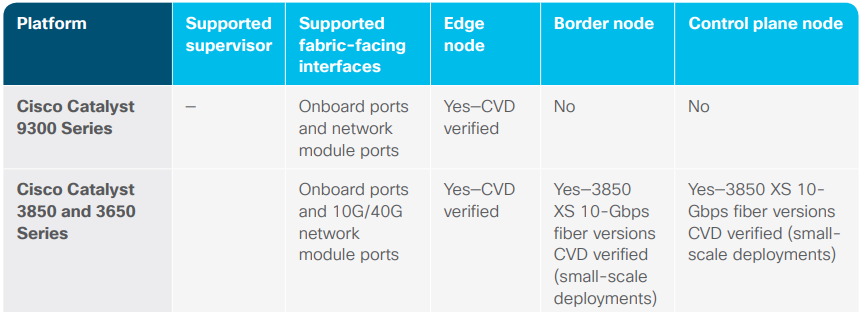
\includegraphics[width=1\linewidth]{img/Analyse/SDAswitchingplatformsanddeploymentcapabilities}
	\caption{SDA switching platforms and deployment capabilities \cite{sda-designguide}}
	\label{fig:SDA switching platforms and deployment capabilities}
\end{figure}

\begin{figure}[H]
	\centering
	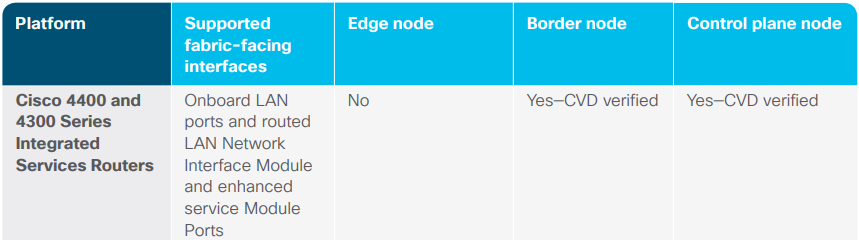
\includegraphics[width=1\linewidth]{img/Analyse/SDAroutingandwirelessplatformsanddeploymentcapabilities}
	\caption{SDA routing and wireless platforms and deployment capabilities \cite{sda-designguide}}
	\label{fig:SDA routing and wireless platforms and deployment capabilities}
\end{figure}

\subsubsection{Grössenüberlegungen}
Es ist zusätzlich zu den oben in den Design Entscheidungen empfohlenen Plattformen wichtig, die nachfolgenden getesteten Werte für Cisco Validated Design (CVD) sowie die Versionshinweise zu Hardware und Software für eine Bereitstellung zu berücksichtigen.

Diese Grössenüberlegungen sind besonders für grosse Unternehmen wichtig, da diese zur Zeit nur bis zur eines gewissen Anzahl von Cisco getestet wurden und im schlechtesten Fall nicht höher unterstützt werden.


\begin{figure}[H]
	\centering
	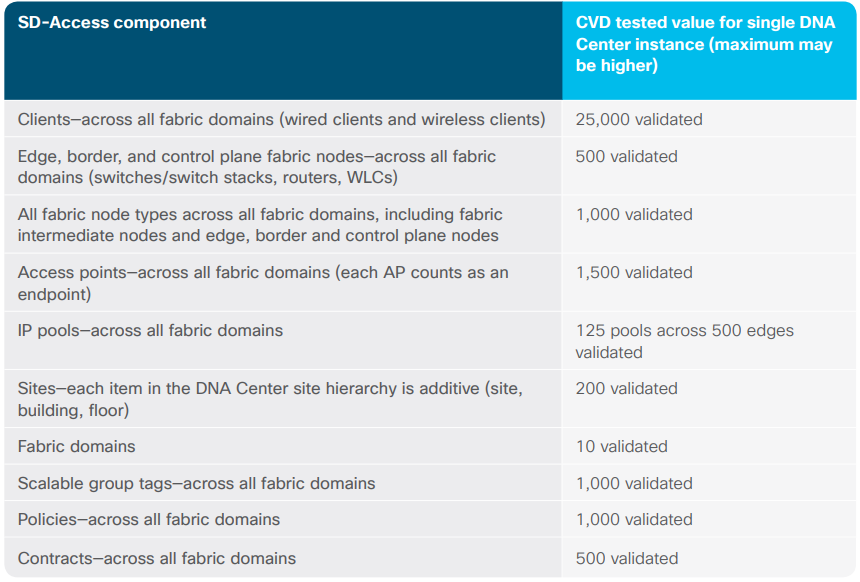
\includegraphics[width=1\linewidth]{img/Analyse/CVD-DNACmanagementofSDA}
	\caption{DNAC management of SDA \cite{sda-designguide} }
	\label{fig:DNAC management of SDA}
\end{figure}

\begin{figure}[H]
	\centering
	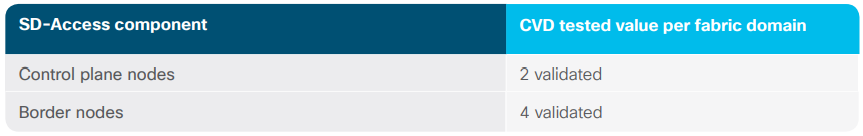
\includegraphics[width=1\linewidth]{img/Analyse/CVD-DNACwithSDAperFabricDomain}
	\caption{DNAC with SDA per each fabric domain \cite{sda-designguide} }
	\label{fig:DNAC with SDA per each fabric domain}
\end{figure}

\begin{figure}[H]
	\centering
	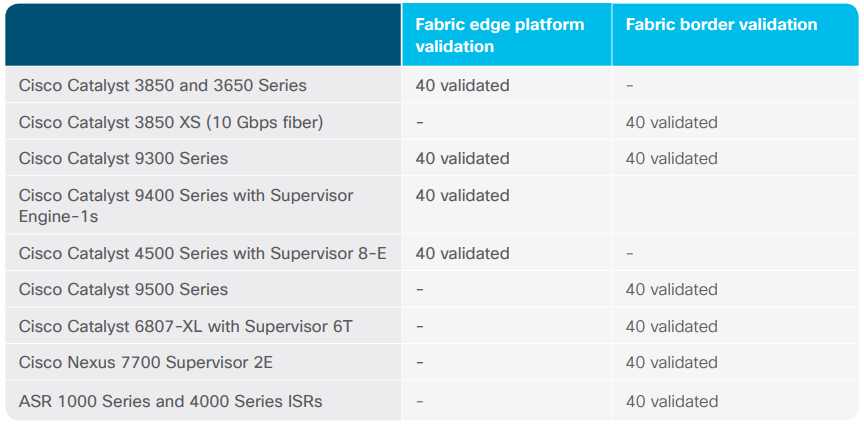
\includegraphics[width=1\linewidth]{img/Analyse/CVD-SDAvirtualnetworksbyplatformandrole}
	\caption{SDA virtual networks by platform and role \cite{sda-designguide} }
	\label{fig:SDA virtual networks by platform and role}
\end{figure}


\subsubsection{Skalierungen}
Folgende maximalen Skalierungen sollten für grosse Organisationen besonders berücksichtigt werden. Diese Daten sollten bei der Auswahl von Plattformen, die während der Planung für das aktuelle und zukünftige Wachstum des Netzwerks verwendet werden, berücksichtigt werden.

Die DNAC Nummern sind pro Instanz, bei denen es sich um ein DNAC mit einem einzelnen Server oder einem DNA-Cluster mit drei Servern handeln kann. Die maximalen Zahlen sind entweder die absoluten Grenzen der Plattform oder die empfohlenen Höchstgrenzen aktueller Tests einer einzelnen Plattform.

\begin{figure}[H]
	\centering
	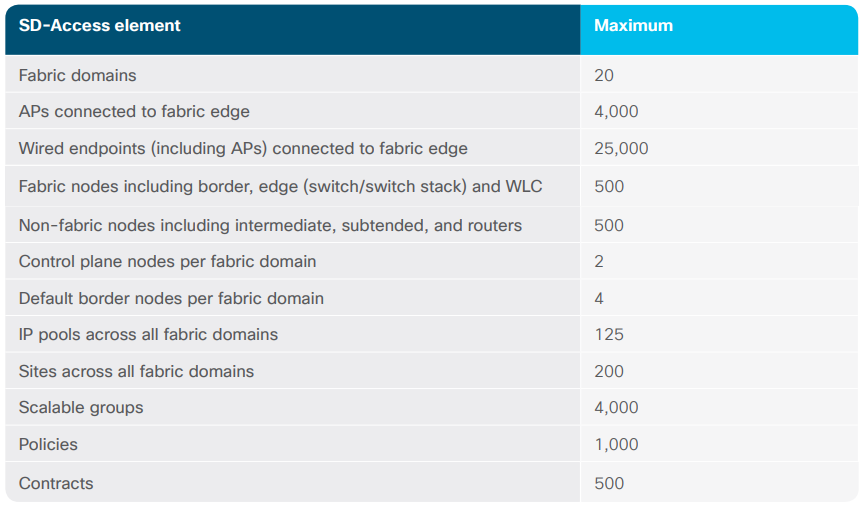
\includegraphics[width=1\linewidth]{img/Analyse/MaxScale-DNAC}
	\caption{DNAC Maximum Scale Recommendations \cite{sda-designguide} }
	\label{fig:DNAC Maximum Scale RecommendationsA}
\end{figure}

\begin{figure}[H]
	\centering
	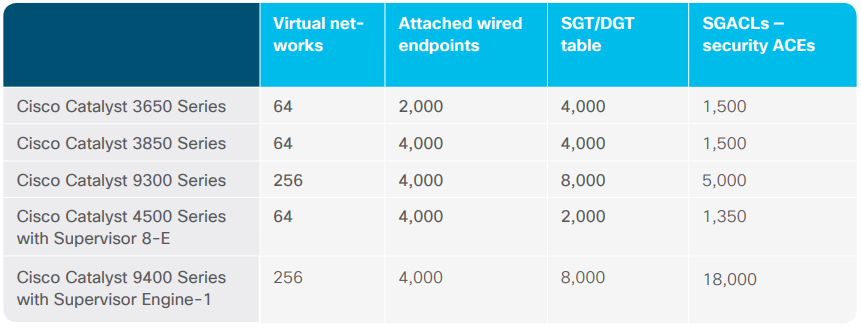
\includegraphics[width=1\linewidth]{img/Analyse/MaxScale-EdgeNode}
	\caption{Edge Node Maximum Scale Recommendations \cite{sda-designguide} }
	\label{fig:Edge Node Maximum Scale RecommendationsA}
\end{figure}

\begin{figure}[H]
	\centering
	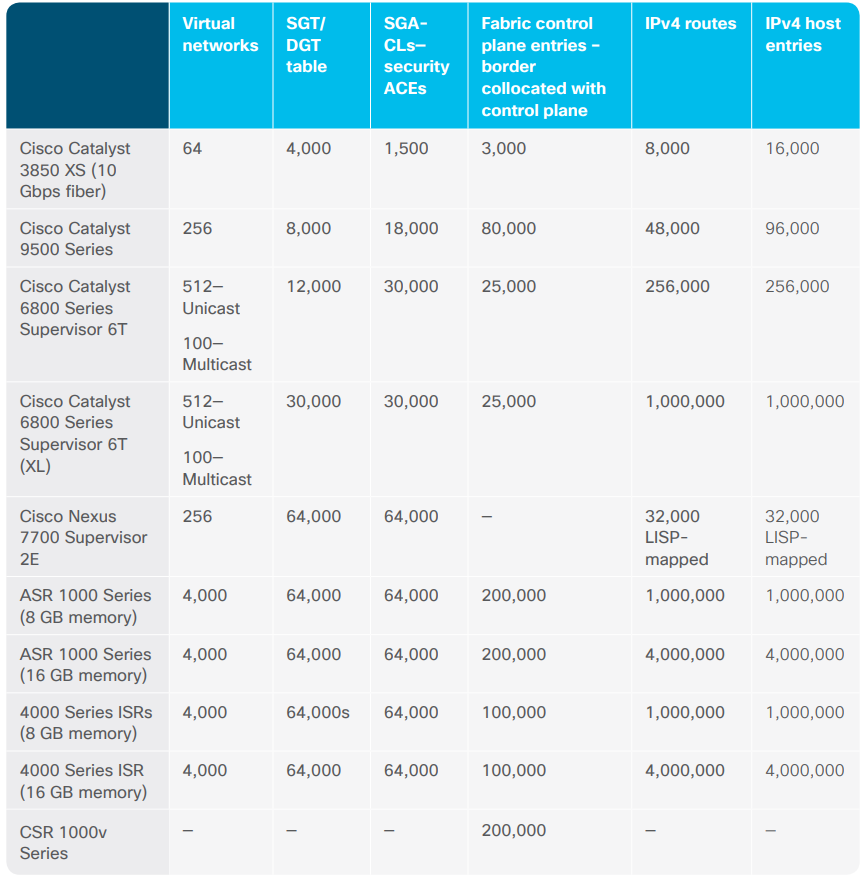
\includegraphics[width=1\linewidth]{img/Analyse/MaxScale-BorderNode}
	\caption{Border Node Maximum Scale Recommendations \cite{sda-designguide} }
	\label{fig:Border Node Maximum Scale RecommendationsA}
\end{figure}




\subsection{Verfügbarkeit}
Die Verfügbarkeit der nachfolgenden Dienste sind für den Betrieb eines SDA mit dem DNAC wichtig, um die volle Funktion des Netzwerkes bereitzustellen. Darum ist es von Vorteil, wenn die kritischen Server und Dienste redundant ausgelegt sind.


\subsubsection{LISP Database}

\subsubsection{Radius}

\subsubsection{SGT Access List}




\subsection{Netzwerk Services}

\subsubsection{NTP}


\subsubsection{DNS}
Der Domain Name Service (DNS) ost eine wesentliche und oft unterschätzte Komponente in einem Netzwerk. Es ist wichtig, dass DNS im Netzwerk korrekt funktioniert und jederzeit zur Verfügung steht.

Es ist also von Vorteil wenn zur Verbeugung eines Ausfalls des DNS, der Server bzw. der Dienst redundant ausgelegt ist.

\subsubsection{Lizenzen}
Die Lizenzen der Geräte können über das DNAC verwaltet werden. Es muss jedoch keine Internetverbindung bestehen, da kein Lizenzenforcement besteht.

\paragraph{Switches}
Die Lizenzen für die einzelnen Switche müssen beim Kauf unbedingt beachtet werden. Jedoch können auf den Switches die Lizenzen auf einer Evaluation Basis manuell nachgerüstet werden (beispielsweise von IP Base auf IP Services).

\subsection{Hardware}
Bei der Hardware ist zu beachten, dass sowohl der Strom, als auch die Netzwerkverbindungen redundant vorhanden sind. Ebenfalls sollte die Hardware bei einem Stromausfall durch eine USV eine gewisse Zeit weiter betrieben werden können.

\paragraph{Wireless Controller}
Die Wireless Controller müssen redundant ausgelegt sein. Es wird in der nachfolgenden Arbeit aber nicht mehr genauer auf Wireless Controller eingegangen, da diese in der Bachelorarbeit nicht integriert werden.


\section{Absicherung}

\subsection{Architektur und Design}
Die SDA Topologie sollte nach den gleichen Designprinzipien und Best Practices aufgebaut werden, welche auch ein Campus-Design verfolgt. Das folgende Beispiel zeigt die physikalische Topologie eines dreistufigen Campus-Designs, bei dem alle Komponenten innerhalb der Fabric redundant sind.

\begin{figure}[H]
	\centering
	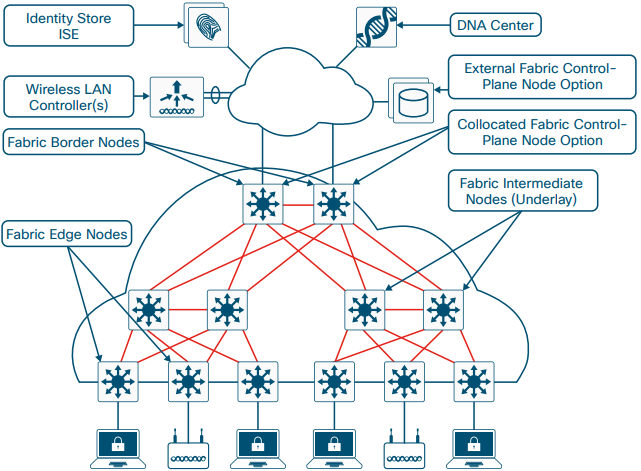
\includegraphics[width=0.8\linewidth]{img/Absicherung/SDA-Architektur}
	\caption{SDA Topologie \cite{sda-designguide-sept2018} }
	\label{fig:SDA Topologie}
\end{figure}

Analog zu dieser wurde die von der Studienarbeit übernommene Architektur weiter angepasst und wenn möglich die Komponenten inklusive Verkabelung redundant ausgelegt (siehe Abbildung \ref{fig:Architektur}: Architektur). \\

Wie in der Analyse festgestellt, sind in der Version 1.2.5 lediglich zwei Control Plane Node unterstützt. Border Nodes könnten maximal vier implementiert werden. Ebenfalls zu beachten sind die Deployment Capabilities, welche als Border und Control Plane Node die Catalyst 3850 empfehlen. Darum werden in der Architektur die Catalyst 9300 als Intermediate oder Edge Nodes eingesetzt.

\subsection{LISP Map Server}
Es gibt zwei Betriebsarten für einen LISP Map-Server(MS): 
\begin{itemize}
	\item als Map-Resolver(MR), der Map-Requests von einem ITR entgegennimmt und das EID-zu-RLOC-Mapping mit Hilfe der verteilten Mapping-Datenbank auflöst
	\item als Map-Server(MS), der autoritative EID-zu-RLOC-Mappings von einem ETR lernt und in der Datenbank veröffentlicht
\end{itemize}

Zur Bereitstellung gibt es zwei Varianten. Zum einem kann es einen redundanten globalen MSMR geben, oder es werden pro Fabric ein MSMR implementiert.

\subsubsection{Redundante MS / MR Bereitstellung}

Es wird empfohlen, redundante Standalone MS- und MR-Systeme mit den MS / MR-Funktionen auf demselben Gerät bereitzustellen. Wenn redundante eigenständige MS / MR implementiert werden, müssen sich alle xTRs bei beiden MS registrieren, so dass jeder eine konsistente Sicht auf den registrierten LISP EID-Namespace hat. Für Map-Resolver-Funktionalität ist die Verwendung einer Anycast-IP-Adresse wünschenswert, da dadurch die Mapping-Lookup-Leistung verbessert wird, indem der MR ausgewählt wird, der dem anfordernden ITR am nächsten ist.

\begin{figure}[H]
	\centering
	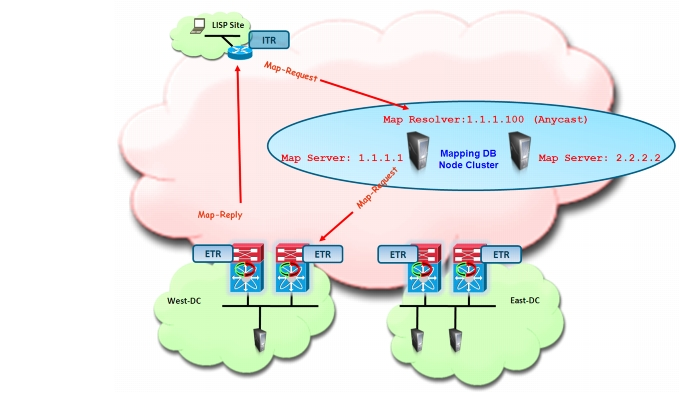
\includegraphics[width=1\linewidth]{img/Absicherung/LISP-Example}
	\caption{Redundante MS / MR Bereitstellung \cite{LISP-mobility} }
	\label{fig:Redundante MS / MR Bereitstellung}
\end{figure}

\subsubsection{Co-Lokalisierung von MS / MR und xTR Funktionalitäten}

Ein weiteres Beispiel ist die Co-Lokalisierung  von MS / MR- und xTR-Funktionalitäten. Das co-lokalisierte Modell ist besonders vorteilhaft, da es die Gesamtzahl verwalteter Geräte reduziert, die zum Ausrollen einer LISP Host Mobility-Lösung erforderlich sind. 

Die erforderliche Konfiguration würde aber in beiden Szenarien identisch bleiben, indem eindeutige IP-Adressen genutzt werden, um die Map-Server und eine Anycast-IP-Adresse für den Map-Resolver zu identifizieren.

\begin{figure}[H]
	\centering
	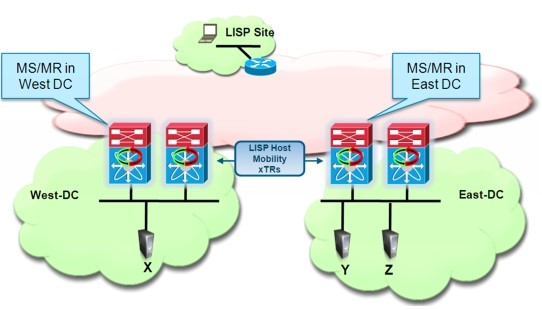
\includegraphics[width=0.8\linewidth]{img/Absicherung/LISP-Example2}
	\caption{Co-Lokalisierung von MS / MR und xTR Funktionalitaeten \cite{LISP-mobility} }
	\label{fig:Co-Lokalisierung von MS / MR und xTR Funktionalitaeten}
\end{figure}

Es kann also ein redundantes eigenständiges MS / MR-Modell bereitgestellt werden, indem dedizierte Systeme zur Durchführung dieser Mapping-Funktionen genutzt werden (siehe Abbildung 2.9) oder alternativ können die MS- und MR-Funktionen gleichzeitig auf dem Netzwerkgerät, welches bereits die xTR-Rolle ausführt, implementiert werden (siehe Abbildung 2.10).

\subsubsection{Anwendung}
Damit bei einem Ausfall eines MSMR nicht alle Fabrics betroffen sind, macht es Sinn pro Fabric einen redundanten MSMR zu implementieren. So können auf einem xTR eine oder mehrere MSMR-Adressen konfiguriert werden.

Abfragen, die ein EID-zu-RLOC-Mapping durchführen, sind datengesteuert. Dieses Verhalten bedeutet, dass ein neuer Datentransfer zwischen LISP-Sites ein Mapping-Lookup erfordert, was dazu führt, dass der Datenversand wird gestoppt, bis ein Mapping durchgeführt wurde. Dies Verhalten ist analog zum DNS-Protokoll und ermöglicht LISP die folgenden Funktionen in einer dezentralen Datenbank mit EID-zu-RLOC-Mappings zu betreiben. 

Die Replikation der gesamten (potenziell umfangreichen) Datenbank ist unnötig, da auf Mappings bei Bedarf zugegriffen wird, genau wie im DNS muss ein Host nicht die komplette Domänendatenbank kennen. Tunnelrouter verwalten den Map-Cache der zuletzt verwendeten Mappings, um die Leistung des Systems zu verbessern.

\paragraph{LISP Client Registration}
Wird ein noch unbekannter neuer Client an die Fabric angeschlossen, sendet der ITR einen Map-Request an einen bekannten MR, wenn es ein EID-zu-RLOC-Mapping benötigt, das noch nicht in seinem lokalen Map-Cache vorhanden ist.

\begin{figure}[H]
	\centering
	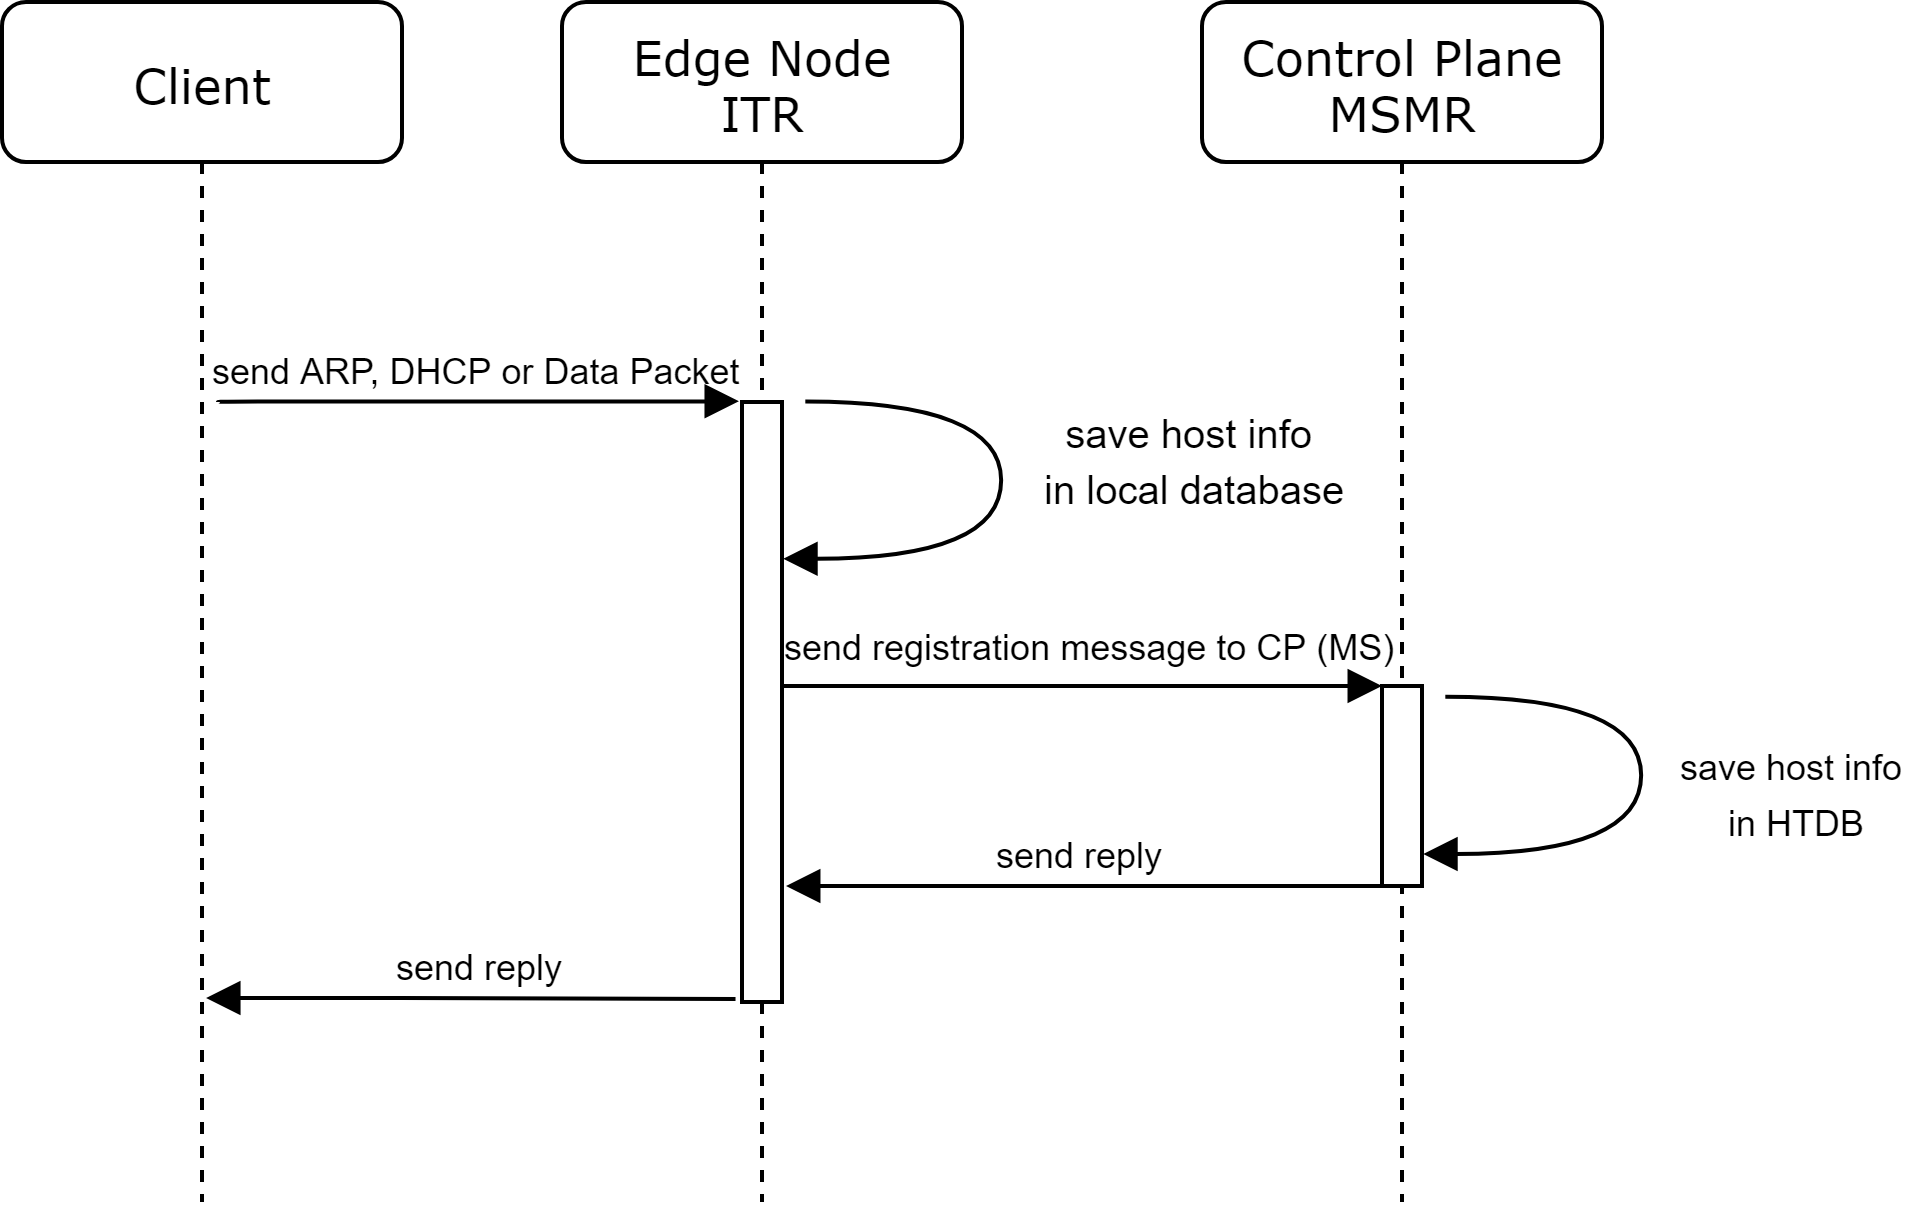
\includegraphics[width=0.8\linewidth]{img/Absicherung/LISP-ClientRegistration}
	\caption{LISP Client Registration}
	\label{fig:LISP Client Registration}
\end{figure}

\paragraph{LISP Host Resolution}
Will ein Client mit einem noch unbekannten anderen Client kommunizieren, so sucht sein ITR zuerst in seinem lokalen Map-Cache nach einem Eintrag. Ist noch kein Eintrag zum Client2 vorhanden, so schickt der ITR ein Map-Request zu seinem MR. Der MS sendet dann den originalen Map-Reguest an den zuletzt registrierten ETR. Da Client2 noch am ETR angeschlossen ist, sendet dieser einen Map-Reply an den ITR, welcher die angefragten Mapping-Informationen enthält.

Bei einem Ping werden die initialen Pakete verworfen, bis die Host Resolution abgeschlossen ist. 

\begin{figure}[H]
	\centering
	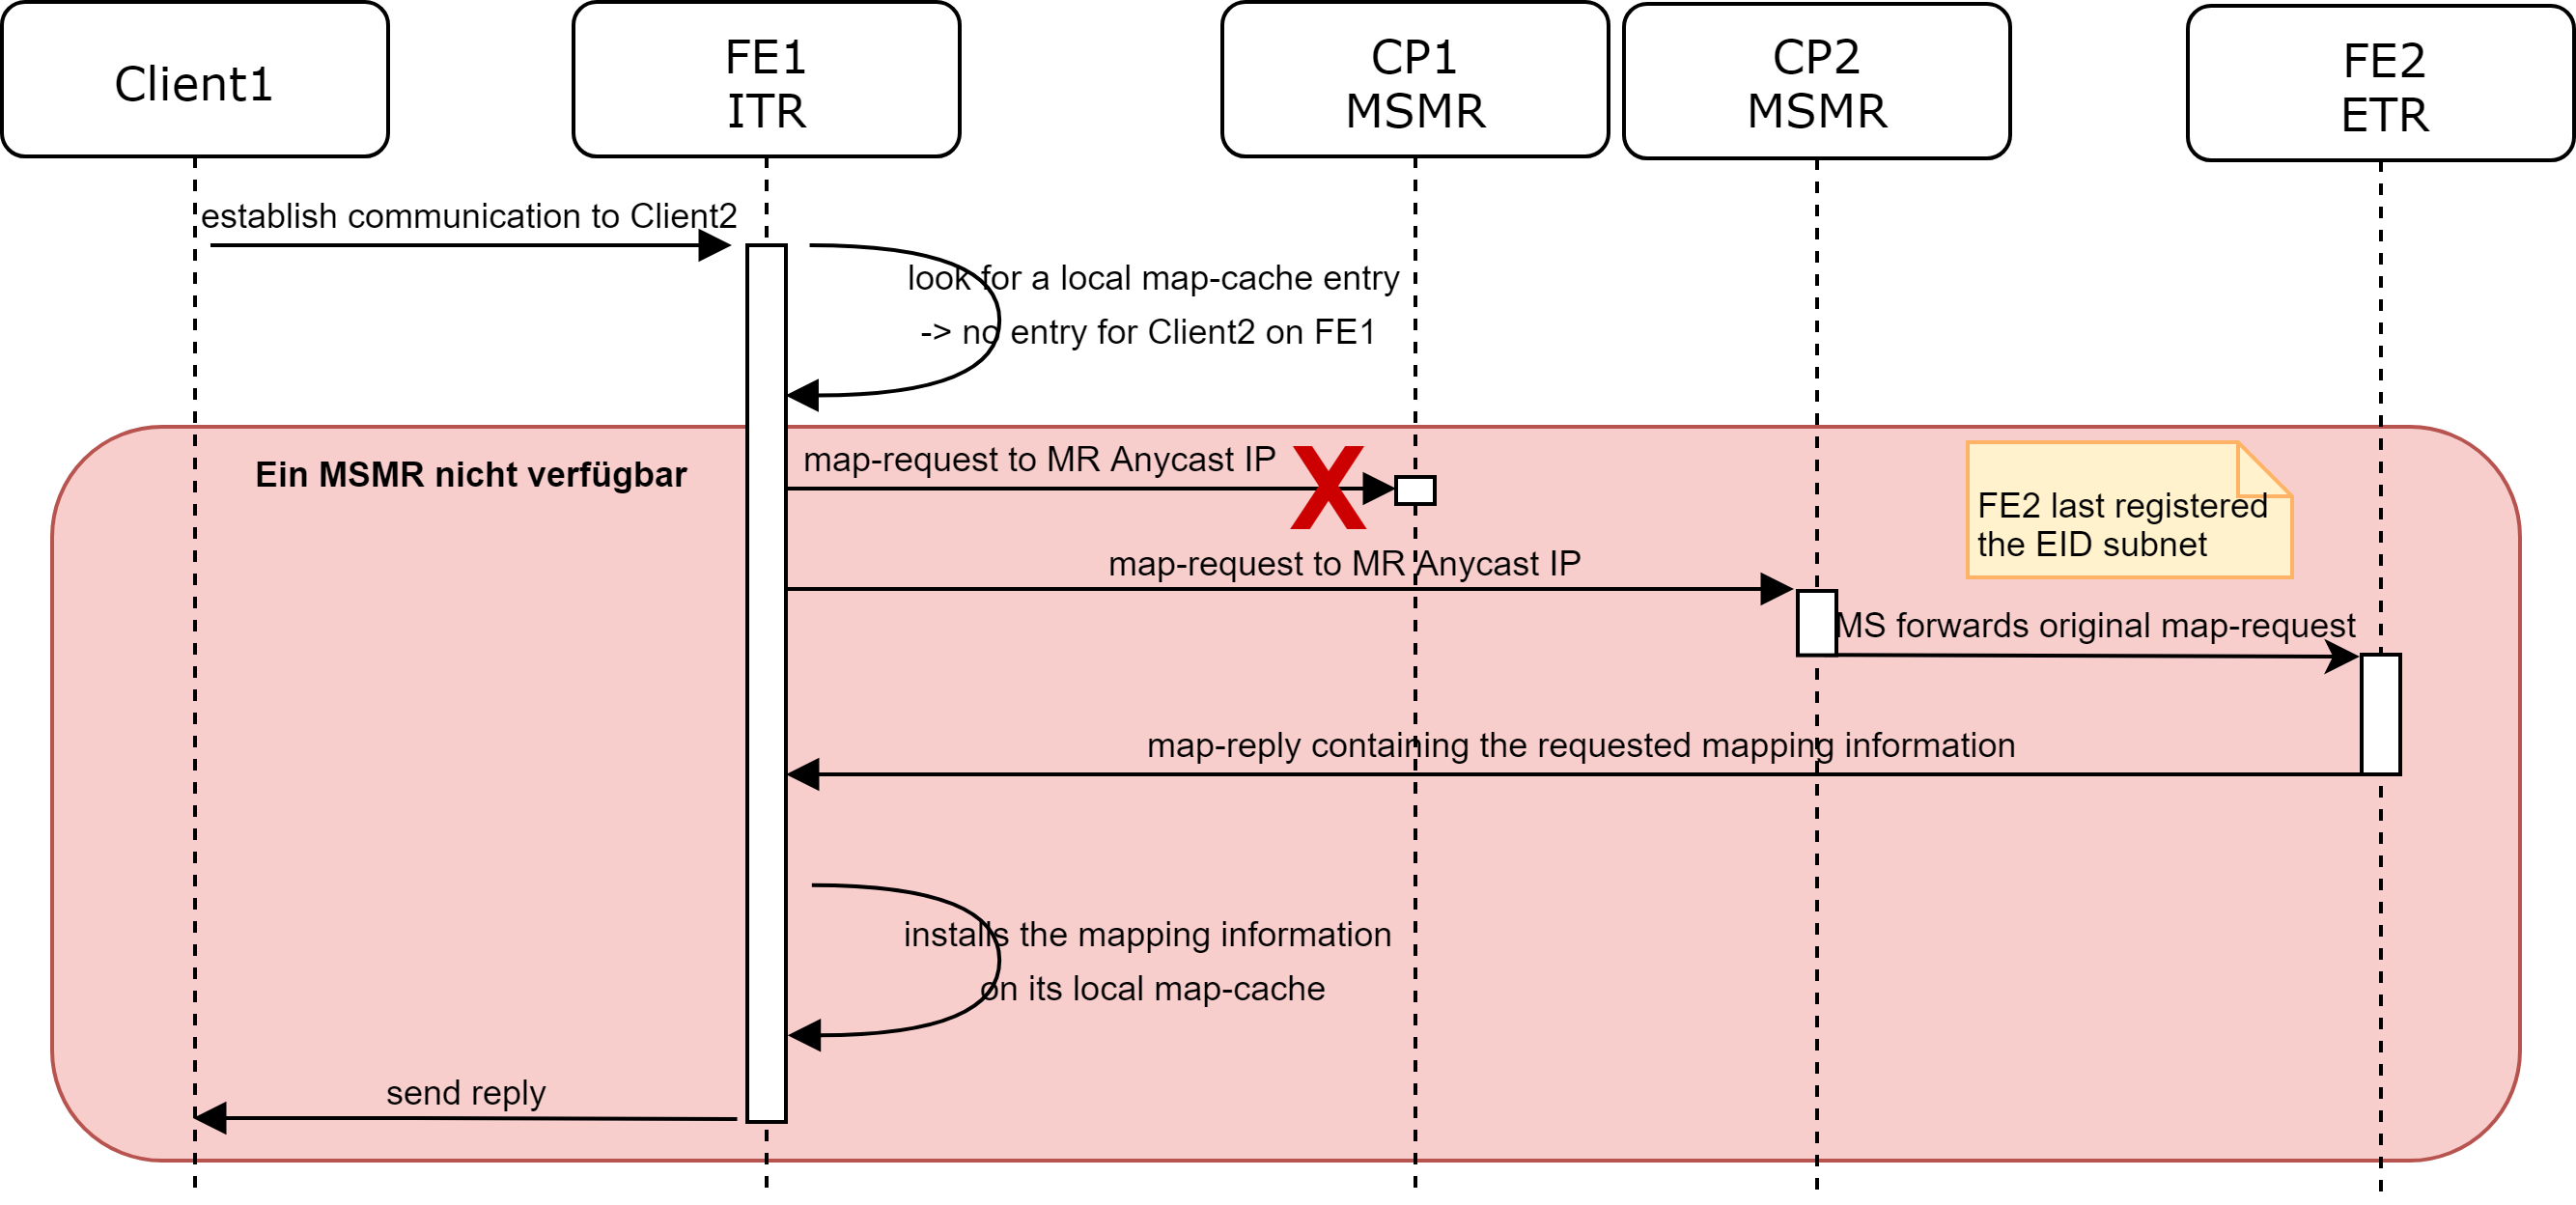
\includegraphics[width=1\linewidth]{img/Absicherung/LISP-HostResolution-Fail}
	\caption{LISP Host Resolution}
	\label{fig:LISP Host Resolution}
\end{figure}

\paragraph{Host Mobility}
Die Host Mobility ist ähnlich wie die Client Registration, da der Client sich beim neuen FE2 zuerst registriert und die neuen Informationen schliesslich vom CP1 dann an den alten FE1 zur Aktualisierung weitergegeben werden.

\begin{figure}[H]
	\centering
	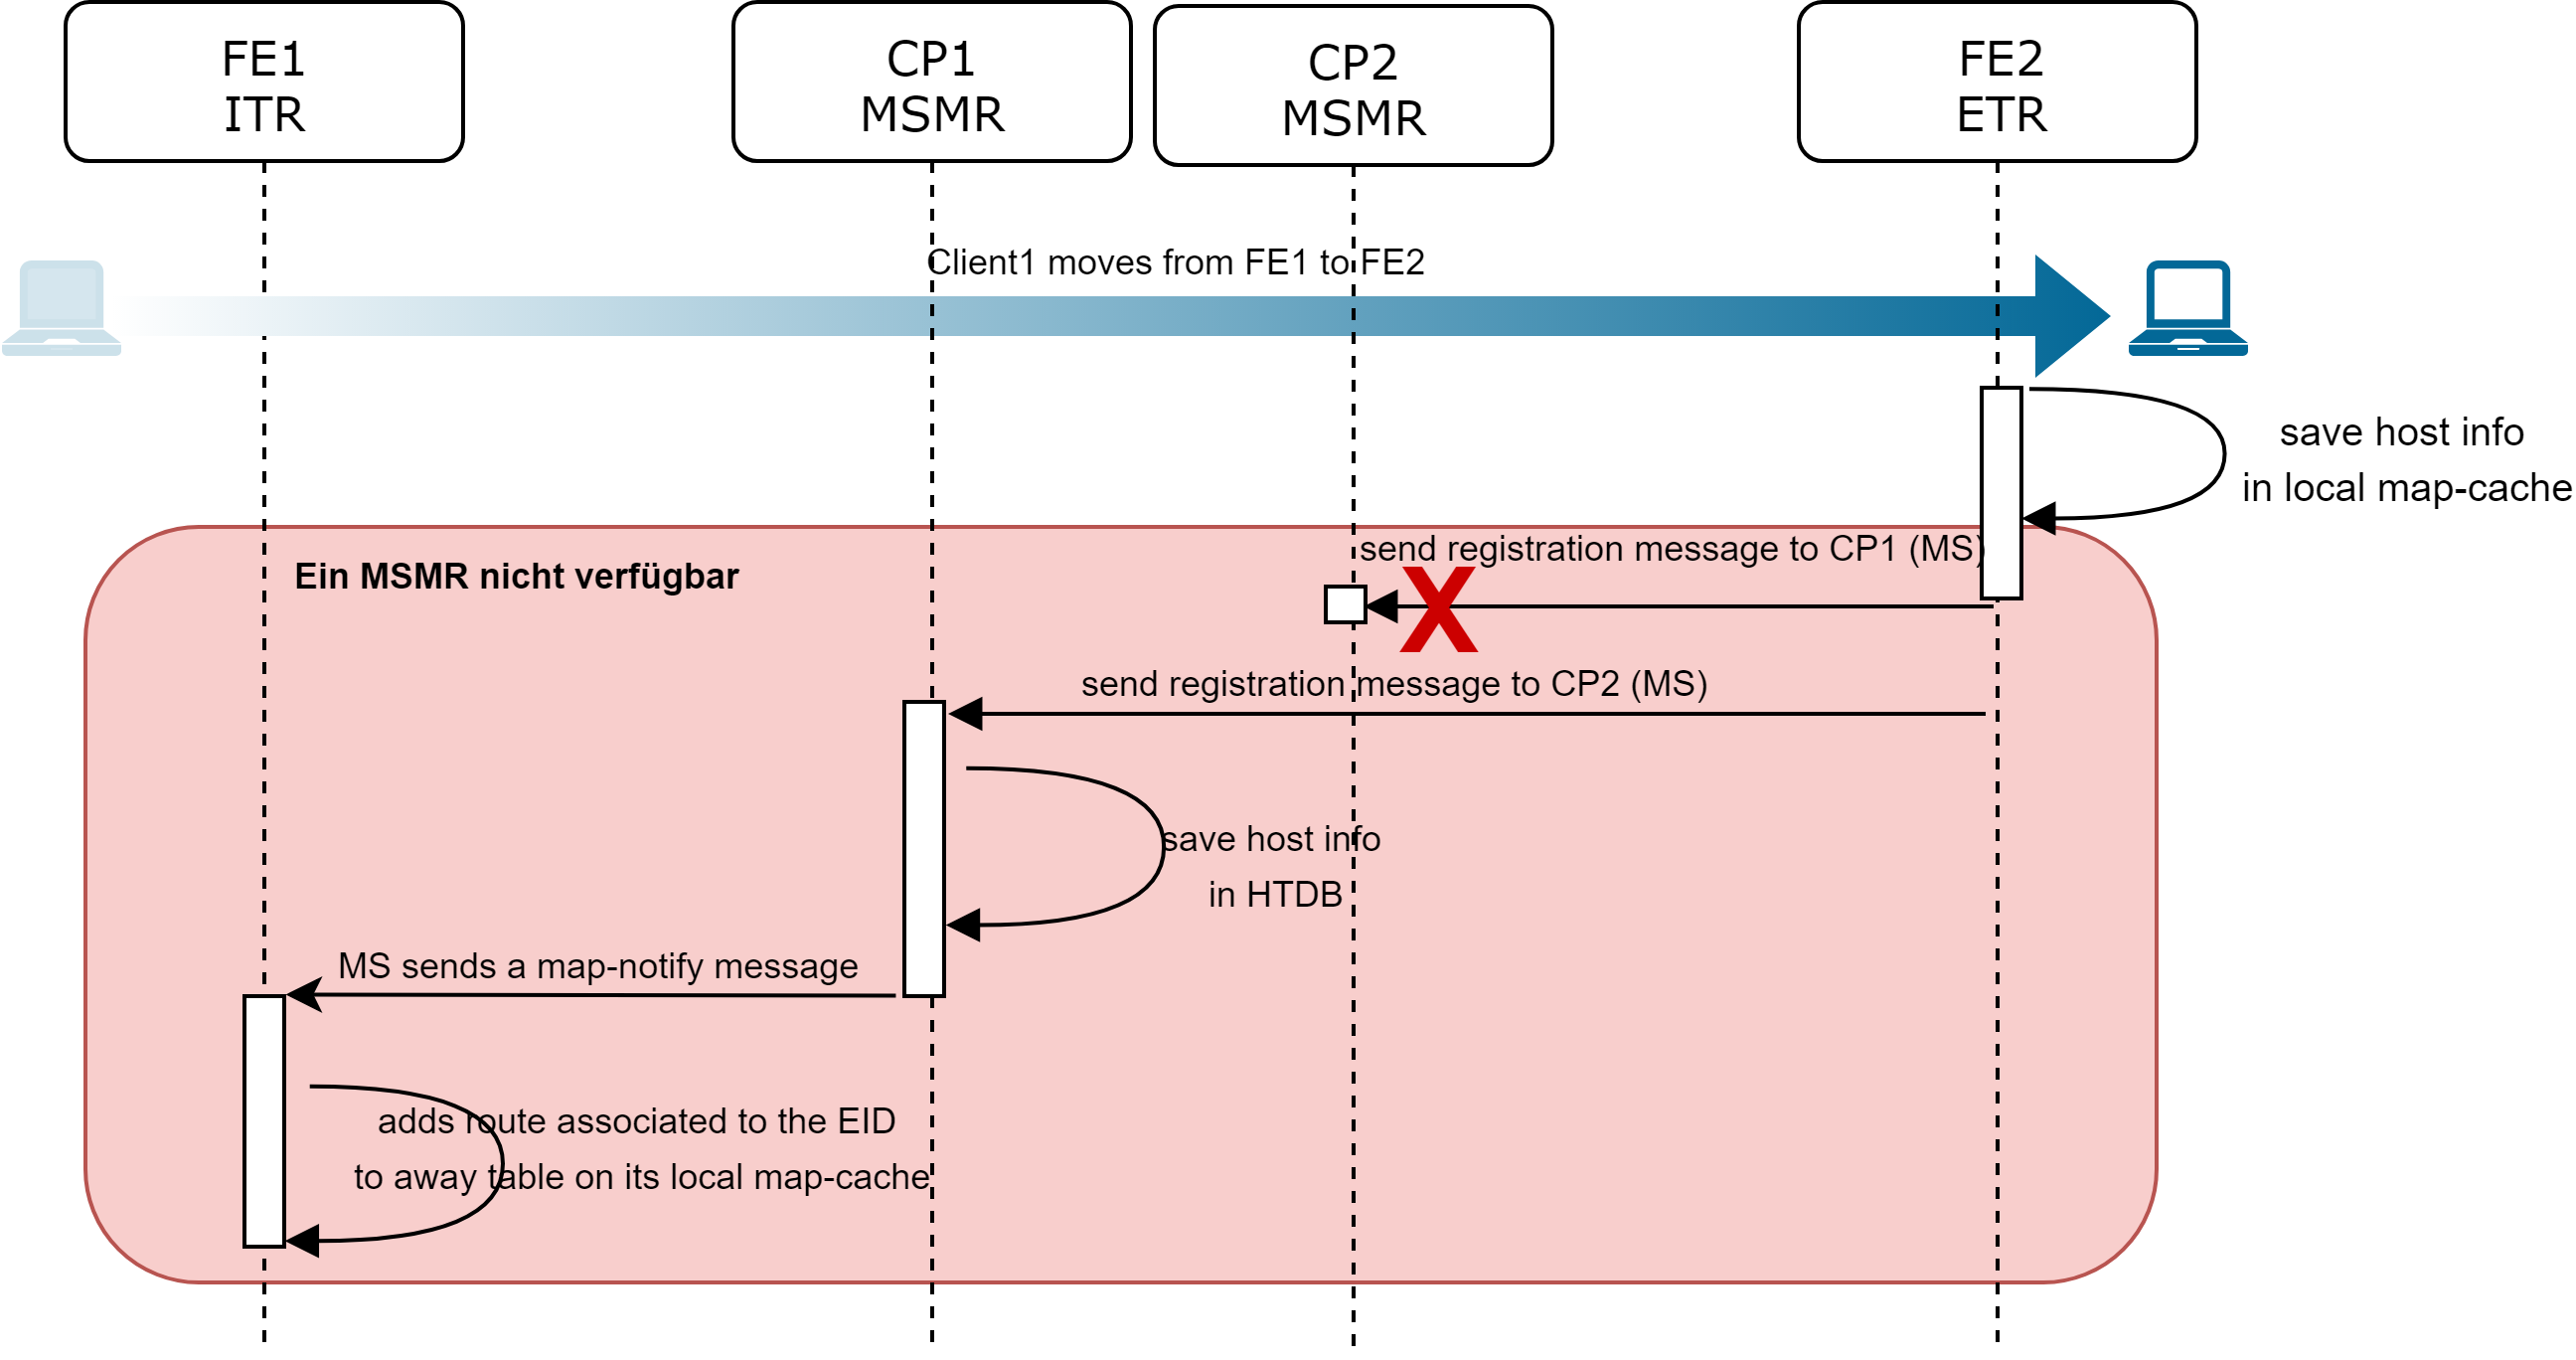
\includegraphics[width=1\linewidth]{img/Absicherung/LISP-HostMobility-Fail}
	\caption{LISP Host Mobility}
	\label{fig:LISP Host Mobility}
\end{figure}

Wenn ein dynamischer EID zwischen Rechenzentrumsstandorten wechselt, müssen die lokalen LISP Host Mobility-xTRs ihre Existenz erkennen. 

Das für LISP Host Mobility konfigurierte xTR erkennt ein Host Mobility Ereignis wenn:
\begin{enumerate}
	\item Er empfängt ein IP-Datenpaket von einer Quelle (des neu eingetroffenen Workloads), die aus Routing-Sicht nicht über die Schnittstelle erreichbar ist, auf der das Paket empfangen wurde.
	\item Die Quelle entspricht der auf die Schnittstelle angewendeten Dynamic-EID-Konfiguration.
\end{enumerate}


\subsubsection{Ausfall MSMR}
Bei einem Ausfall des MSMR kann keine Host Registration mehr vorgenommen werden. Das heisst neue Clients können keine Verbindung zum restlichen Netzwerk aufbauen. Bestehende Clients können nur mit Clients welche am selben FE angeschlossen sind kommunizieren. Dies jedoch nur solange ihr Eintrag im lokalen Map-Cache bestehen bleibt. Der TTL der Einträge im Map-Cache beträgt per default einen Tag. 

Da jeder xTR seinen eigenen Map-Cache hat und kann sich sein Inhalt innerhalb derselbe LISP-Site unterscheiden. Daher können xTr leicht schwere Paketausfälle erleiden und mit LISP Control Messages geflutet werden.  

\paragraph{MS}
Es sollten mehrere Map-Server vorhanden und eingetragen sein. Sollte der erste Map-Server nicht erreichbar sein, so wird der zweite Map-Server verwendet.

\paragraph{MR}
Für den Map-Resolver sollte eine Anycast IP-Adresse verwendet werden. So werden die Pakete gesendet und über einen verfügbaren Map-Resolver zum Ziel weitergeleitet.

\subsection{ISE / Radius}

\subsubsection{ISE Cluster}

Um die Verfügbarkeit des ISE zu erhöhen, kann diese in einem Cluster, bestehend aus einem Master und mehreren Slaves betrieben werden. Dies erhöht die Ausfallsicherheit aller Services auf dem ISE. Damit diese gewährleistet sind, wenn ein Aussenstandort die Verbindung zum Hauptsitz verliert, müsste aber an jedem Standort ein ISE Slave existieren. Bei sehr vielen Standorten ist dies auf Grund des Verwaltungsaufwands und der Kosten für viele ISE Instanzen nicht praktikabel. Ein Cluster am Hauptstandort ist aber sicherlich sinnvoll.

\subsubsection{Read Only Radius Server an Aussenstandorten}

In Aussenstellen wird ein Read Only Radius Server betrieben, damit die Network Access Devices auch im Falle eines Unterbruchs der Verbindung zum Hauptsitz einen Radius Server zur Verfügung haben. Hier könnte beispielsweise Freeradius eingesetzt werden. Da Freeradius seine Informationen nicht direkt vom ISE beziehen kann, muss vom ISE ein externer Radius Server verwendet werden, der eine Replikation unterstützt. Dies kann beispielsweise Freeradius sein.

\paragraph{ISE}


\paragraph{Freeradius}

Freeradius wird in einem Master / Slave Setup betrieben. Am Hauptstandort befindet sich der Radius Master und an allen Aussenstandorten ist ein Slave verfügbar. Die Replikation wird mittels MySQL Replikation sichergestellt.

\paragraph{Network Access Devices}

Auf den Network Devices muss der Radius Server vom jeweiligen Standort konfiguriert sein. Dies kann im DNA Center unter \textit{Design $\rightarrow$ Network Settings $\rightarrow$ AAA Server} konfiguriert werden.

\begin{figure}[H]
	\centering
	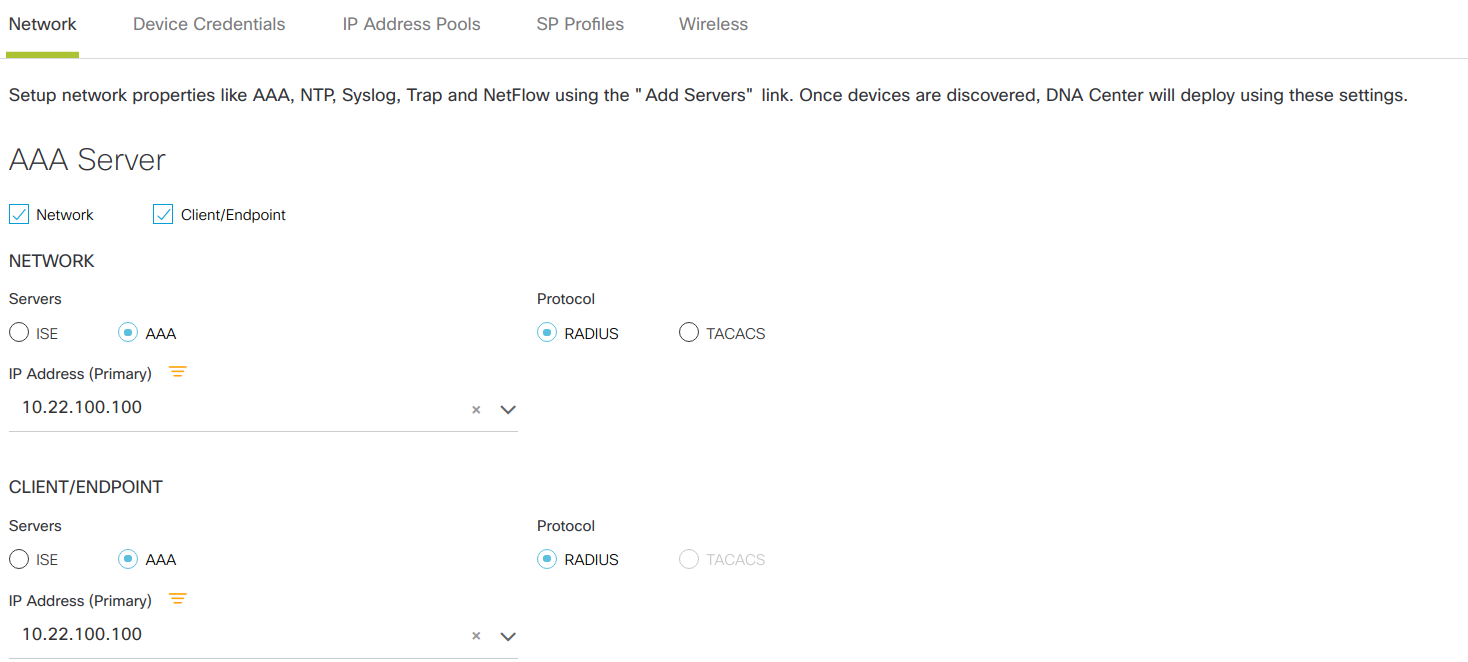
\includegraphics[width=0.8\linewidth]{img/Absicherung/DNA_Center_AAA-Server.png}
	\caption{DNA Center - AAA Server }
	\label{fig:DNA Center - AAA Server}
\end{figure}


\subsection{SGT Access List}
Beim Erstellen von SGTs über die DNAC-Benutzeroberfläche wird die ISE-Benutzeroberfläche cross-gestartet und die Aufgabe wird dort abgeschlossen. ISE verwaltet alle skalierbaren Gruppeninformationen, die später in DNAC für die Richtlinienerstellung verwendet werden. Obwohl die Richtlinien und die entsprechenden Verträge bei DNAC erstellt werden, werden beide über die REST-API der ISE an die ISE zurückgemeldet. ISE dient dann als zentrale Anlaufstelle für SGTs, Richtlinien und Verträge (SGACLs), die dann dynamisch an die Netzwerkinfrastruktur verteilt werden.
Die Segmentierung innerhalb der SDA wird durch die kombinierte Verwendung von virtuellen Netzwerken (VN), die mit VRFs gleichgesetzt sind, als auch TrustSec Scalable Group Tags (SGTs) ermöglicht. Während die Segmentierung durch die Verwendung von absichtsgesteuerten oder speziell dafür entwickelten virtuellen Netzwerken allein erreicht werden kann, bieten die Cisco Trustsec SGTs eine logische Segmentierung basierend auf der Gruppenmitgliedschaft. Cisco bietet eine zusätzliche Granularitätsebene, mit der mehrere SGTs innerhalb eines einzigen VN verwenden können, die eine Mikrosegmentierung innerhalb des VN ermöglicht. Die Segmentierung erfolgt innerhalb des SDA sowohl auf Makro- als auch auf Mikroebene durch virtuelle Netzwerke bzw. SGTs. Die Richtlinien und die damit verbundenen Verträge werden im DNAC konfiguriert und dann über die REST-API an die ISE übermittelt. ISE aktualisiert dann die Edge Nodes mit nur den Richtlinien für SGTs, die den angeschlossenen Geräten zugeordnet sind. Die Durchsetzung erfolgt beim Austritt, wenn das Ziel verbunden ist. \cite{sda-segmentation-may2018}

Kurze Zusammenfassung der damit benötigten Komponenten:
\begin{itemize}
	\item Sicherheitsgruppe (SG) - Eine Gruppe von Benutzern, Endpunktgeräten und Ressourcen, die Zugriffssteuerungsrichtlinien gemeinsam nutzen. SGs werden vom Administrator in Cisco ISE definiert. Wenn neue Benutzer und Geräte zur TrustSec Domäne hinzugefügt werden, ordnet Cisco ISE diese neuen Entitäten den entsprechenden Sicherheitsgruppen zu.
	\item Security Group Tag (SGT) - Der TrustSec-Dienst weist jeder Sicherheitsgruppe eine eindeutige 16-Bit-Sicherheitsgruppennummer zu, deren Gültigkeitsbereich innerhalb einer TrustSec Domäne global ist. Die Anzahl der Sicherheitsgruppen im Switch ist auf die Anzahl der authentifizierten Netzwerkentitäten beschränkt. Die Sicherheitsgruppennummern müssen nicht manuell konfigurieren. Sie werden automatisch generiert, aber es gibt auch die Möglichkeit eine Reihe von SGTs für die IP-zu-SGT-Zuordnung zu reservieren.
	\item Security Group Access Control List (SGACL) - Mit SGACLs kann der Zugriff und die Berechtigung basierend auf den zugewiesenen SGTs gesteuert werden. Die Gruppierung von Berechtigungen in einer Rolle vereinfacht die Verwaltung von Sicherheitsrichtlinien. Beim Hinzufügen von Geräten wird einfach eine oder mehrere Sicherheitsgruppen zugewiesen und diese erhalten sofort die entsprechenden Berechtigungen. Die Sicherheitsgruppen können geändert werden, um neue Berechtigungen einzuführen oder die aktuellen Berechtigungen einzuschränken.
	\item Security Exchange Protocol (SXP) - Das SGT Exchange Protocol (SXP) ist ein Protokoll, das für den TrustSec Dienst entwickelt wurde, um die IP-SGT-Bindungen auf Netzwerkgeräte zu übertragen, die keine SGT-fähige Hardwareunterstützung für Hardware bieten, die SGT / SGACL unterstützt.
\end{itemize}


\begin{figure}[H]
	\centering
	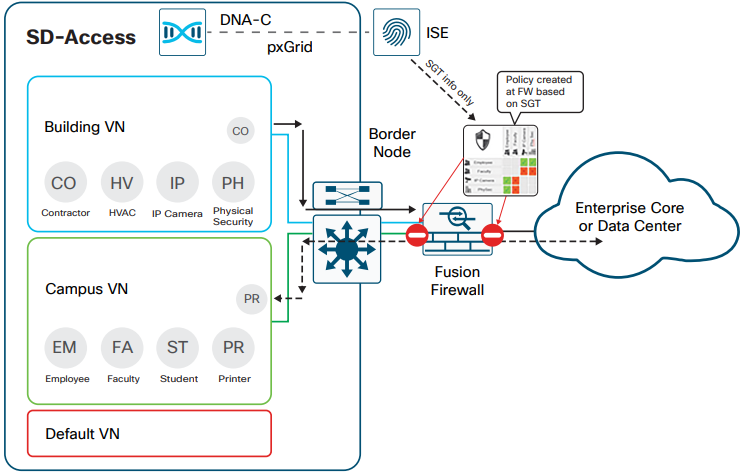
\includegraphics[width=1\linewidth]{img/Absicherung/SGT-FusionFirewall}
	\caption{Policy Enforcement mit einer Fusion Firewall}
	\label{fig:Policy Enforcement mit einer Fusion Firewall}
\end{figure}

Oben dargestellte Abbildung veranschaulicht die Verwendung einer Fusion Firewall, welche für die Kommunikation zwischen virtuellen Netzwerken sowie für den Verkehr an einem anderen Ort im Netzwerk. Mithilfe von Standard ACLs oder gruppenbasierten Richtlinien mit SGTs werden Firewall-Regeln in der Fusions-Firewall definiert, die den Datenverkehr zwischen Endpunkten steuert.

\subsubsection{Failover}
Die Absicherung der Access Listen kann beispielsweise nach folgenden Beispielen erarbeitet werden, müssen jedoch noch genauer getestet werden:

\begin{itemize}
	\item Beispiel1: lokal auf 9300 SGACLs alle fünf Minuten sichern und diese bei Ausfall wieder eintragen. Nachteil: Host-Mobility funktioniert nicht, aber lokal kann weitergearbeitet werden.
	\item Beispiel2: global komplett alle SGACLs auf alle Geräte verteilen. Vorteil: Alle Geräten haben jederzeit alle Einträge. Nachteil: Die Maximum Scale Recommendations der SGACLs sind pro Gerät anders. C3850 - 1500 SGACLs, C9300 - 5000 SGACLs
\end{itemize}

Es können TrustSec SXP Speaker/Listener auf den Catalyst 3850 und C9300 definiert werden, indem die Catalyst 3850 als Gateway für die Catalyst 9300 Listener angegeben werden.

Der Timeout der SGACL Caches beträgt per default zwei Minuten. Dieser könnte auch unendlich viel höher gesetzt werden, jedoch würde man nicht mehr merken, wenn ein Ausfall eines Gerätes vorliegt. Die Suche nach der Fehlerquelle würde sich enorm erschweren.

\subsection{Border Node}

Der gesamte Verkehr der die Fabric betritt oder verlässt, durchläuft diesen Knoten. Um einen Single Point of Failure zu vermeiden, sollten immer mindestens zwei Border Nodes pro Fabric zur Verfügung stehen. Nach aktuellen Maximum Scale Recommendations können maximal 4 Border Nodes pro Fabric Domain implementiert werden.

Border Nodes implementieren die folgenden Funktionen, welche bei einem Ausfall in Mitleidenschaft gezogen werden könnten\cite{sda-designguide-sept2018}:
\begin{itemize}
	\item Ankündigung von EID-Subnetzen
	\item Fabric-Domänenausstiegspunkt
	\item Mapping der LISP-Instanz auf VRF
	\item Richtlinienzuordnung
\end{itemize}

\subsubsection{Ankündigung von EID-Subnetzten}
SD-Access konfiguriert Border Gateway Protocol (BGP) als bevorzugtes Routingprotokoll, das für die Ankündigung der EID-Präfixe außerhalb der Fabric verwendet wird, und der für EID-Subnetze von außerhalb der Fabric bestimmte Verkehr wird durch die Grenzknoten geleitet. Diese EID-Präfixe werden nur in den Routingtabellen am Rand angezeigt. Im gesamten Rest der Fabric wird auf die EID-Informationen über die Fabric-Steuerebene zugegriffen.

\subsubsection{Fabric-Domänenausstiegspunkt}
Der externe Fabric Border ist das Gateway des letzten Auswegs für die Fabric Edge Nodes. Dies wird mithilfe der LISP Proxy Tunnel Router-Funktionalität implementiert. Möglich sind auch interne Fabric Borders, die mit Netzwerken mit einem genau definierten Satz von IP-Subnetzen verbunden sind, wodurch die Ankündigung dieser Subnetze in der Fabric hinzugefügt werden muss.

\subsubsection{Mapping der LISP-Instanz auf VRF}
Der Fabric Border Node kann die Netzwerkvirtualisierung mithilfe von externen VRF-Instanzen von innerhalb der Fabric auf die Fabric-Außenseite ausweiten, um die Virtualisierung beizubehalten.

\subsubsection{Richtlinienzuordnung}
Der Fabric Border Node bildet auch SGT-Informationen aus der Fabric ab, die beim Verlassen dieser Fabric entsprechend verwaltet werden. SGT-Informationen werden vom Fabric Border Node an das ausserhalb der Fabric liegende Netzwerk weitergegeben, indem entweder die Tags mithilfe von SGT Exchange Protocol (SXP) zu Cisco-fähigen Geräten transportiert werden, oder indem SGTs direkt in einem Cisco-Metadatenfeld in einem Paket zugeordnet werden Inline-Tagging-Funktionen für Verbindungen zum Grenzknoten implementiert.

\subsection{Fusion Router}
Die Fusion Router stellen die Verbindungen zwischen den einzelnen Fabrics, dem Internet, sowie die Verbindung zum Legacy Netzwerk in dem sich beispielsweise das DNAC und der ISE befinden.Es werden mehrere Fusion Router verwendet, um die nötige Ausfallsicherheit zu gewährleisten. Die Fusion Router und Border Nodes sind im Optimalfall in einem Full-Mesh verkabelt. Für das Routing zwischen den Fusion Routern, sowie den Border Nodes kommt BGP zum Einsatz.

Die Topologie wurde analog anhand der nachfolgenden Validation Topologie von Cisco aufgebaut.
\begin{figure}[H]
	\centering
	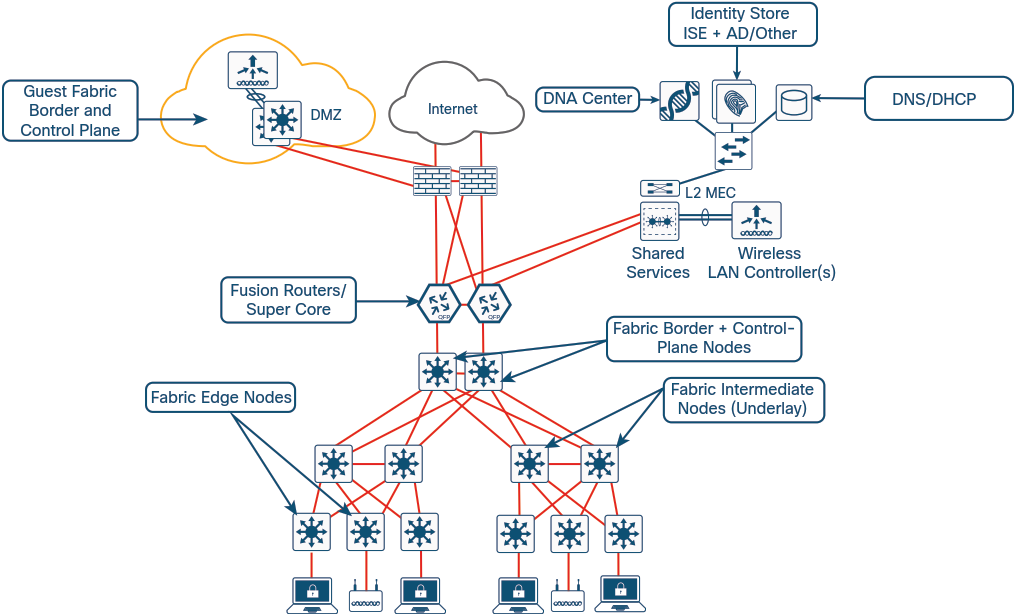
\includegraphics[width=1\linewidth]{img/Absicherung/FusionRouter-ValidationTopology}
	\caption{Fusion Router Validation Topology \cite{sda-deploymentguide-oct2018} }
	\label{fig:Fusion Router Validation Topology}
\end{figure}


\subsection{DHCP}

\subsubsection{Infoblox}
Um die Krisenresistenz am Hauptstandort zu erhöhen, wird Infoblox als Multi-Node Cluster betrieben. Dadurch kann ein einzelner Node ausfallen, ohne dass dies einen Impact auf den Betrieb am Hauptstandort hat. 

\subsubsection{Aussenstellen}
Da sich Infoblox nicht in Kombination mit 3rd Party Software in einem Cluster oder einer Failoverlösung betreiben lässt, müssen an Aussenstandorten eigenständige DHCP Server betrieben werden, um deren Autonomie sicherzustellen. Da Infoblox den isc-dhcp-server für seine DHCP Services verwendet, wird dieser auch an den Aussenstellen eingesetzt. 
Für wichtige Aussenstandorte kann der isc-dhcp-server in einem Master-Slave Cluster betrieben werden. Somit isch an diesen Standorten ebenfalls eine Ausfallsicherheit gewährleistet.

\subsubsection{DNA Center}
Im DNA Center muss für jeden Aussenstandort der jeweilige DHCP Server konfiguriert werden. Im Falle eines DHCP Clusters können hier auch mehrere Einträge erstellt werden.

\begin{figure}[H]
	\centering
	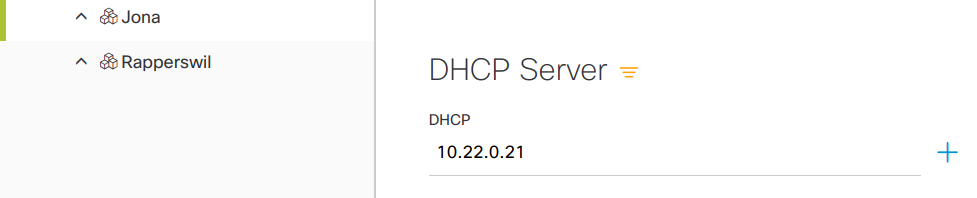
\includegraphics[width=0.8\linewidth]{img/Absicherung/DNA_Center_DHCP-Server.png}
	\caption{DNA Center - DHCP Server }
	\label{fig:DNA Center - DHCP Server}
\end{figure}

\subsection{DNS}

\subsubsection{Infoblox HA Cluster}


\subsubsection{Read Only DNS Server an Aussenstandorten}
	
Damit Aussenstellen nicht auf DNS Server des Hauptstandortes angewiesen sind, kann in jedem Standort ein Read-Only Server betrieben werden. Somit funktioniert die Namensauflösung auch im Falle eines Kommunikationsverlusts zum Hauptstandort. 

\begin{figure}[H]
	\centering
	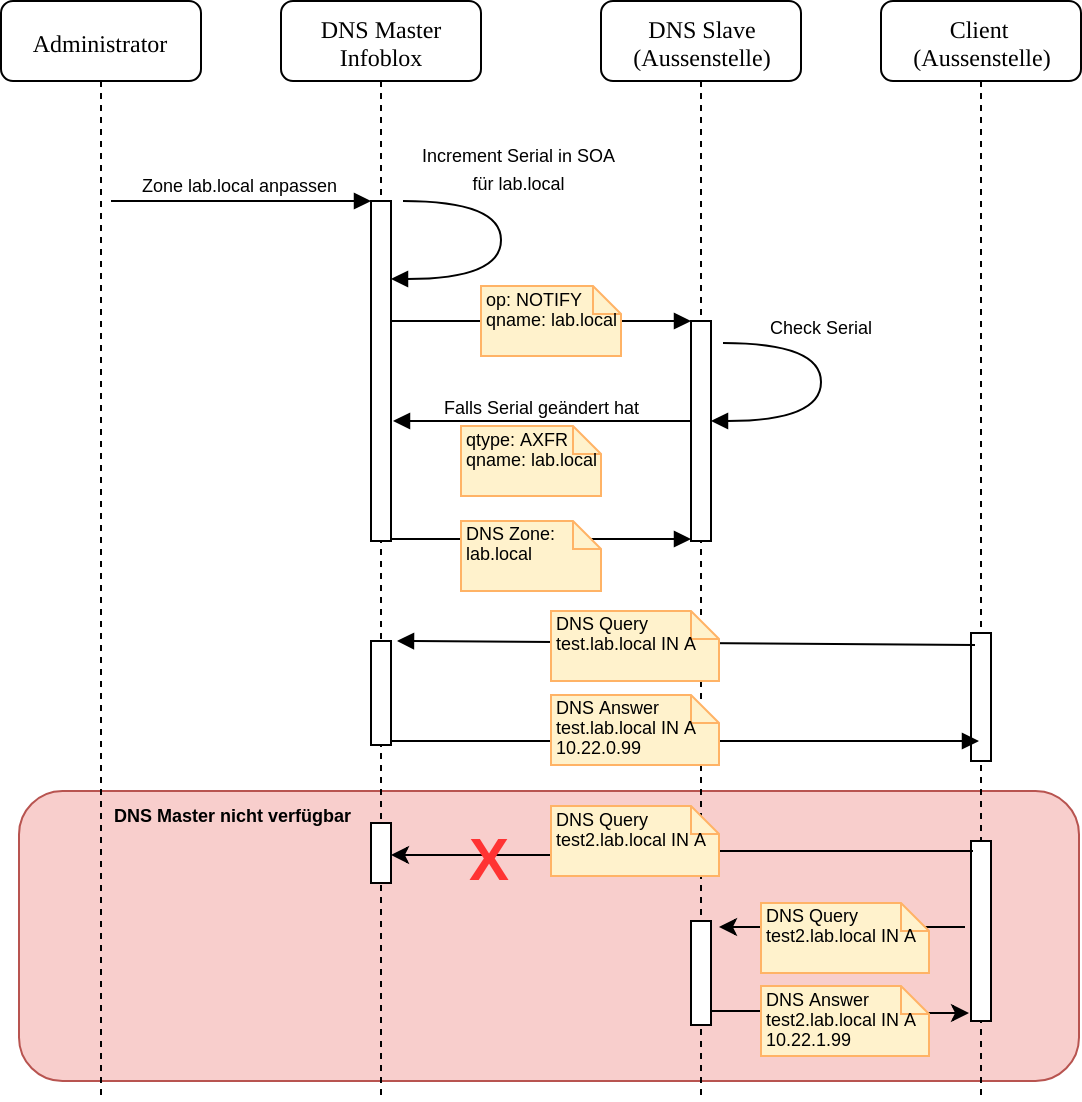
\includegraphics[width=0.8\linewidth]{img/Absicherung/DNS_Sequenzdiagram.png}
	\caption{DNS Sequenzdiagramm}
	\label{fig:DNS Sequenzdiagramm}
\end{figure}
\paragraph{Infoblox}

Damit die Read-Only Server stets über die aktuellsten DNS Zonen verfügen, müssen die Informationen von Infoblox auf diese repliziert werden. In diesem Fall wird dafür der Zone Transfer verwendet. Dazu muss dies in Infoblox für alle Slave Server erlaubt werden. 

Dies wird in Infoblox via \textit{Grid $\rightarrow$ DNS $\rightarrow$ Infoblox Instanz $\rightarrow$ Edit $\rightarrow$ Zone Transfers} ausgeführt.

\begin{figure}[H]
	\centering
	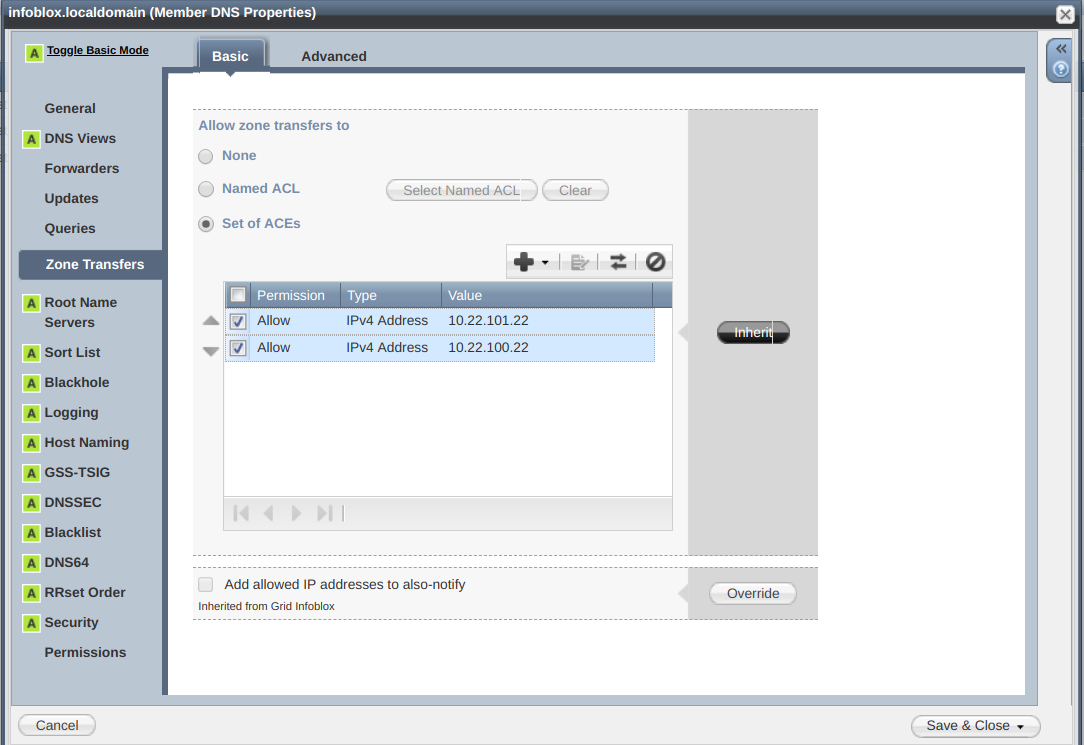
\includegraphics[width=0.8\linewidth]{img/Absicherung/Infoblox_Zone_Transfer.png}
	\caption{Infoblox Zone Transfer}
	\label{fig:Infoblox Zone Transfer}
\end{figure}

\paragraph{DNS Slaves}

Auf den Slaves an den jeweiligen Aussenstandorten müssen die Zonen als Slave Zonen konfiguriert sein und Infoblox muss als Master konfiguriert werden. Dadurch können die Zonen vom Master auf den Slave transferiert werden. Der Slave aktualisiert alle Slave Zonen in regelmässigen Abständen. Dieser Intervall wird in der Zone im SOA Record mit dem "Refresh" Parameter definiert.
Zusätzlich kann auf dem Master konfiguriert werden, dass alle Slaves mittels "Notify" informiert werden, sobald sich eine Zone ändert, worauf der Slave die aktuellsten Informationen für diese Zone abruft. Somit ist sichergestellt, dass alle Server an Aussenstandorten stets über eine aktuelle Konfiguration verfügen.

\paragraph{Clients}

Auf den Cliens ist es wichtig, dass alle nötigen DNS Server in der korrekten Reihenfolge konfiguriert werden. Als erster Server soll der Master, also Infoblox eingetragen werden. Sofern Infoblox als Cluster betrieben wird, können auch alle Instanzen des Clusters verwendet werden. Danach der Slave am jeweiligen Standort. Dies sorgt dafür, dass der Slave nur dann verwendet wird, wenn die Kommunikation zum Master nicht funktioniert.
\section{Abstrahierung}

Im nachfolgenden Teil wird die Umsetzung der folgenden Use Cases beschrieben. Die Use Cases sind nach der Nummerierung priorisiert worden. Der UC01 soll auf jeden Fall umgesetzt werden. Der UC02 muss evaluiert werden, ob dies mit der API des DNA Centers im Zusammenspiel mit dem ENCS überhaupt möglich ist. Zum Schluss kommt der UC03, welcher nur optional ist und bei genügend verbleibender Zeit implementiert wird.

\subsection{Use Cases Brief}

\subsubsection{UC01: Network Orchestration}
Ein Administrator kann in einem Web Interface Netzwerke erstellen und verwalten. Des Weiteren ist die Möglichkeit gegeben, Policies, welche die Kommunikation zwischen diesen Netzen regeln zu erstellen. Die entsprechenden Konfigurationen werden auf allen beteiligten Geräten automatisch via APIs erstellt.

\subsubsection{UC02: ENCS Virtual Machine Management}
Ein Administrator kann in einem Web Interface die VMs auf einem ENCS System verwalten.

\subsubsection{UC03: Configuration History}
Ein Web Interface bietet die Möglichkeit, die Konfigurationen aller Geräte innerhalb einer Fabric anzuzeigen. Des weiteren kann die aktuelle Konfiguration mit älteren Versionen der Konfiguration verglichen werden.

\subsection{Use Cases Fully Dressed}

\subsubsection{UC01: Network Orchestration}
\begin{table}[H]
	\rowcolors{2}{gray!25}{white}
	\centering
	\begin{tabularx}{\textwidth}{l | X}
		Primary Actor      & Administrator        \\
		\hline
		Beschreibung       & Ein Administrator kann in einem Web Interface Netzwerke erstellen und verwalten. Des Weiteren ist die Möglichkeit gegeben, Policies, welche die Kommunikation zwischen diesen Netzen regeln zu erstellen. Die entsprechenden Konfigurationen werden auf allen beteiligten Geräten automatisch via APIs erstellt. \\ 
		\hline
		Stakeholders       &  
		\begin{itemize}	
			\item Administrator
			\item User
		\end{itemize}              \\
		\hline
		Preconditions      & 
		\begin{itemize}	
			\item DNA Center komplett konfiguriert
			\item Die Fabric läuft ohne Einschränkung
			\item Web Interface steht zur Verfügung
		\end{itemize}  \\
		\hline
		Postconditions     & 
		\begin{itemize}	
			\item Änderungen an Netzen wurden auf den Netzwerkdevices umgesetzt
			\item Policies sind korrekt umgesetzt
		\end{itemize}  \\
		\hline
		Main Success Story & 
		\begin{enumerate}
			\item Ein Netzwerk wird erstellt
			\item Die Software erstellt das Netzwerk auf allen nötigen Netzwerkgeräten
			\item Eine Policy für die Kommunikation mit anderen Netzen wird definiert
			\item Die Konfiguration für die Policy wird automatisch auf allen nötigen Netzwerkgeräten erstellt
		\end{enumerate}
		\\
		\hline
		Alternative Flows  & 
		\begin{itemize}
			\item[1a.] Ein Netzwerk wird gelöscht
			\item[1b.] Eine Policy wird verändert
		\end{itemize}
	\end{tabularx}
	\caption{UC01 Fully Dressed}
	\label{tab:UC01}
\end{table}

\subsubsection{UC02: ENCS Virtual Machine Management}
\begin{table}[H]
	\rowcolors{2}{gray!25}{white}
	\centering
	\begin{tabularx}{\textwidth}{l | X}
		Primary Actor      & Administrator        \\
		\hline
		Beschreibung       & Ein Administrator kann in einem Web Interface die VMs auf einem ENCS System verwalten. \\ 
		\hline
		Stakeholders       &  
		\begin{itemize}	
			\item Administrator
		\end{itemize}              \\
		\hline
		Preconditions      & 
		\begin{itemize}	
			\item ENCS ist konfiguriert und mit dem DNA Center verbunden
			\item VM Profile existieren
		\end{itemize}  \\
		\hline
		Postconditions     & 
		\begin{itemize}	
			\item VMs befinden sich im gewünschten Zustand
		\end{itemize}  \\
		\hline
		Main Success Story & 
		\begin{enumerate}
			\item Eine VM wird erstellt
			\item Eine VM wird gestartet
			\item VM wird einem Netzwerk zugewiesen
		\end{enumerate}
		\\
		\hline
		Alternative Flows  & 
		\begin{itemize}
			\item[1a.] VM wird gelöscht
		\end{itemize}
	\end{tabularx}
	\caption{UC02 Fully Dressed}
	\label{tab:UC02}
\end{table}

\subsubsection{UC03: Configuration History}
\begin{table}[H]
	\rowcolors{2}{gray!25}{white}
	\centering
	\begin{tabularx}{\textwidth}{l | X}
		Primary Actor      & Administrator        \\
		\hline
		Beschreibung       & Ein Web Interface bietet die Möglichkeit, die Konfigurationen aller Geräte innerhalb einer Fabric anzuzeigen. Des weiteren kann die aktuelle Konfiguration mit älteren Versionen der Konfiguration verglichen werden. \\ 
		\hline
		Stakeholders       &  
		\begin{itemize}	
			\item Administrator
		\end{itemize}              \\
		\hline
		Preconditions      & 
		\begin{itemize}	
			\item Netzwerkgeräte sind erreichbar
		\end{itemize}  \\
		\hline
		Postconditions     & 
		\begin{itemize}	
			\item Konfiguration wird angezeigt
		\end{itemize}  \\
		\hline
		Main Success Story & 
		\begin{enumerate}
			\item Ein Netzwerkgerät wird gewählt
			\item Ein Zeitpunkt wird gewählt
			\item Konfiguration zum gewählten Zeitpunkt kann mit der aktuellen Version verglichen werden
		\end{enumerate}
		\\
		\hline
		Alternative Flows  & 
	\end{tabularx}
	\caption{UC03 Fully Dressed}
	\label{tab:UC03}
\end{table}

\subsection{Technologien}
Für das entwickeln des Orchestrierungstool wird Python verwendet. Für das Web Interface wird das Framework Flask eingesetzt. Mit diesen Technologien wird eine Web Anwendung entwickelt, die mit Hilfe der APIs des DNA Centers, des ENCS und der Netzwerkgeräte einzelne Prozesse vereinfacht oder automatisiert.

\subsubsection{Python}
Python ist eine objektorientierte Programmiersprache. Die einfache und leicht erlernbare Python-Syntax hebt die Lesbarkeit hervor und reduziert dadurch die Programmwartung. Python unterstützt Module und Pakete, was die Modularität von Programmen und die Wiederverwendung von Code fördert. Der Python-Interpreter und die umfangreiche Standardbibliothek sind in Quell- oder Binärform kostenlos für alle gängigen Plattformen verfügbar und können frei verteilt werden. \cite{python}

\subsubsection{Flask}
Flask ist ein in Python geschriebenes Webframework. Der Fokus von Flask liegt auf Erweiterbarkeit und guter Dokumentation. Die einzigen Abhängigkeiten sind Jinja2, eine Template-Engine und Werkzeug, eine Bibliothek zum Erstellen von WSGI-Anwendungen. \cite{flask}

\subsubsection{DNA Center Platform}
Cisco hat seit dem Sommer 2018 die DNA Center Platform zur Verfügung gestellt, über die nun auf den API Katalog und andere Ressourcen zugegriffen werden kann. So können beispielsweise die Platform Funktionen auch verwendet werden, um die Bereitstellung und Verwaltung von Netzwerken zu vereinfachen.


So soll das DNA Center nun eine 360 Grad Erweiterbarkeit durch vier verschiedene Platform Funktionen bereitstellen. Dazu gehören die Intent-based APIs, Process adapters, Domain adapters, sowie SDKs. \cite{dnac-platform}

\begin{figure}[H]
	\centering
	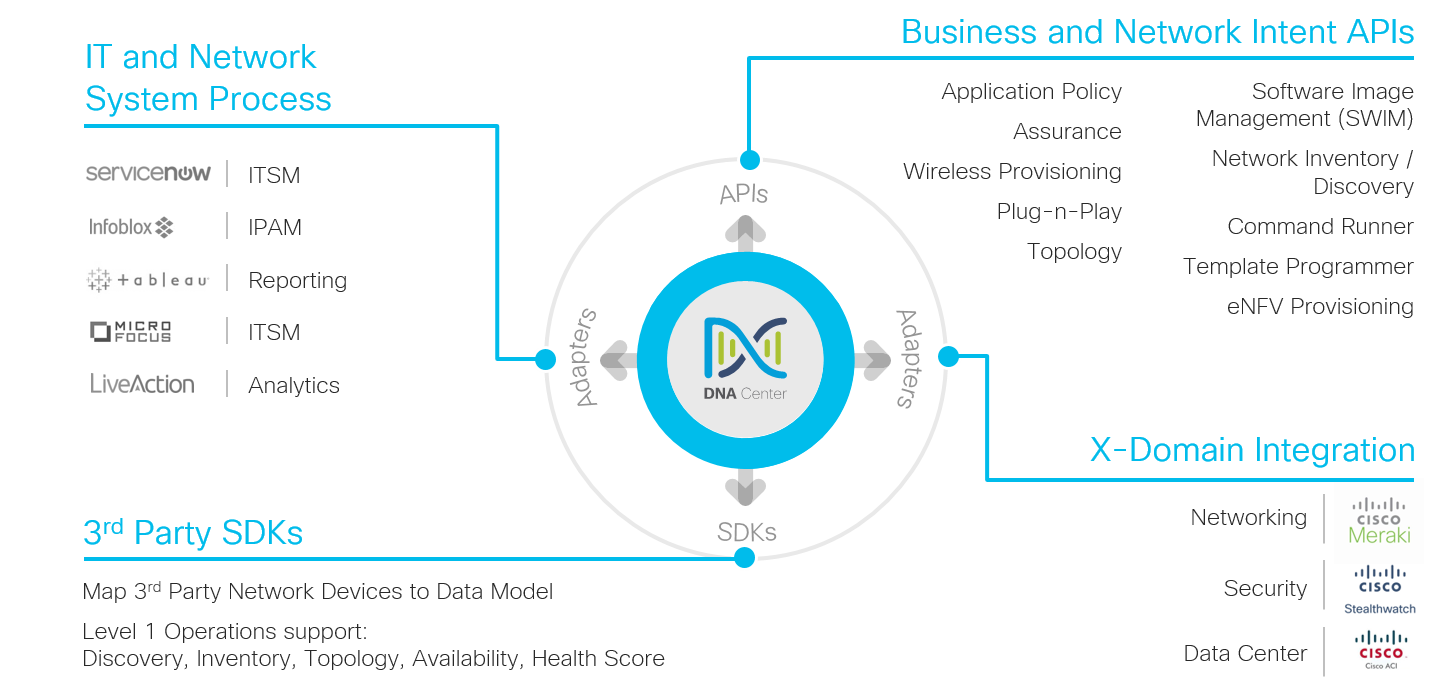
\includegraphics[width=0.8\linewidth]{img/Abstrahierung/dnac-platform}
	\caption{DNA Center Plattform \cite{dnac-platform}}
	\label{fig:DNA Center Plattform}
\end{figure}


\paragraph{Intent-API}

Die Intent-API ist eine Northbound REST API, welche bestimmte Funktionen des DNA Centers verfügbar macht. Mit der RESTful Intent API des DNA Centers können die HTTP- (GET, POST, PUT, DELETE) und JSON-Syntax verwendet werden, um das Netzwerk zu analysieren und zu konfigurieren. \cite{dnac-platform}

Diese APIs findet man im DNA Center unter \textit{Platform $\rightarrow$ Developer Toolkit $\rightarrow$ APIs}

\begin{figure}[H]
	\centering
	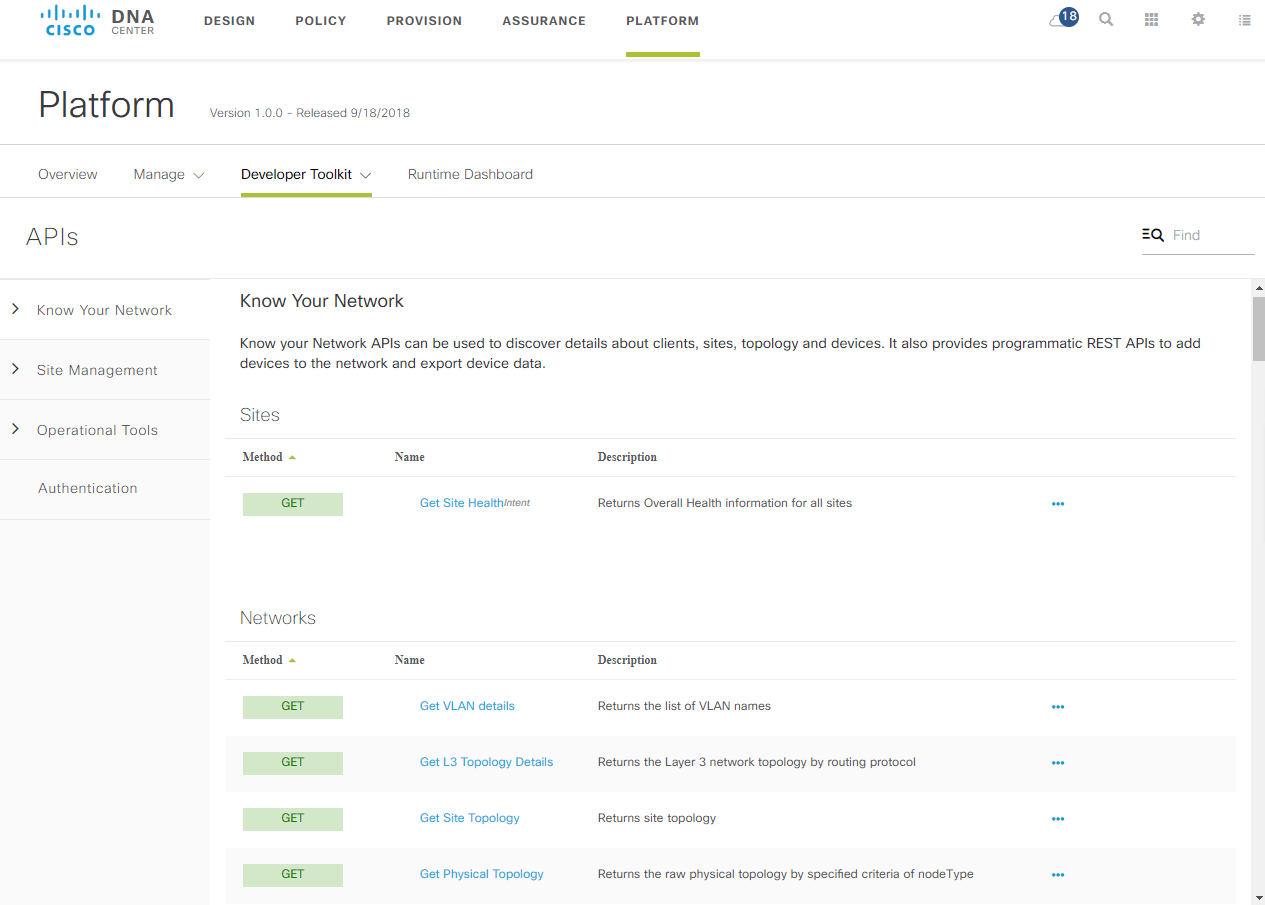
\includegraphics[width=0.8\linewidth]{img/Abstrahierung/dnac-apis}
	\caption{DNA Center Plattform APIs}
	\label{fig:DNA Center Plattform APIs}
\end{figure}

\subsubsection{ENCS/NFVIS API}
Der ENCS beziehungsweise die NFVIS, welche auf dem ENCS läuft, stellt ebenfalls eine programmierbare API für Service Orchestration mittels REST- und NETCONF-API bereit. 

Die API Dokumentationen sind bei NFVIS leider nicht direkt über dessen Applikation verfügbar. Es gibt jedoch eine Dokumentation von Cisco direkt, welche unter dem Namen \textit{API Reference for Cisco Enterprise Network Function Virtualization Infrastructure Software} \cite{nfvis-api} zu finden ist.


\subsection{Umsetzung}

\subsubsection{Ablauf Erstellung Netzwerk}
Um die Erstellung eines Netzwerkes zu vereinfachen, wird ein Wizard erstellt, mit welchem folgende einzelnen Schritte vereinfacht auszuführen sind. 

\begin{figure}[H]
	\centering
	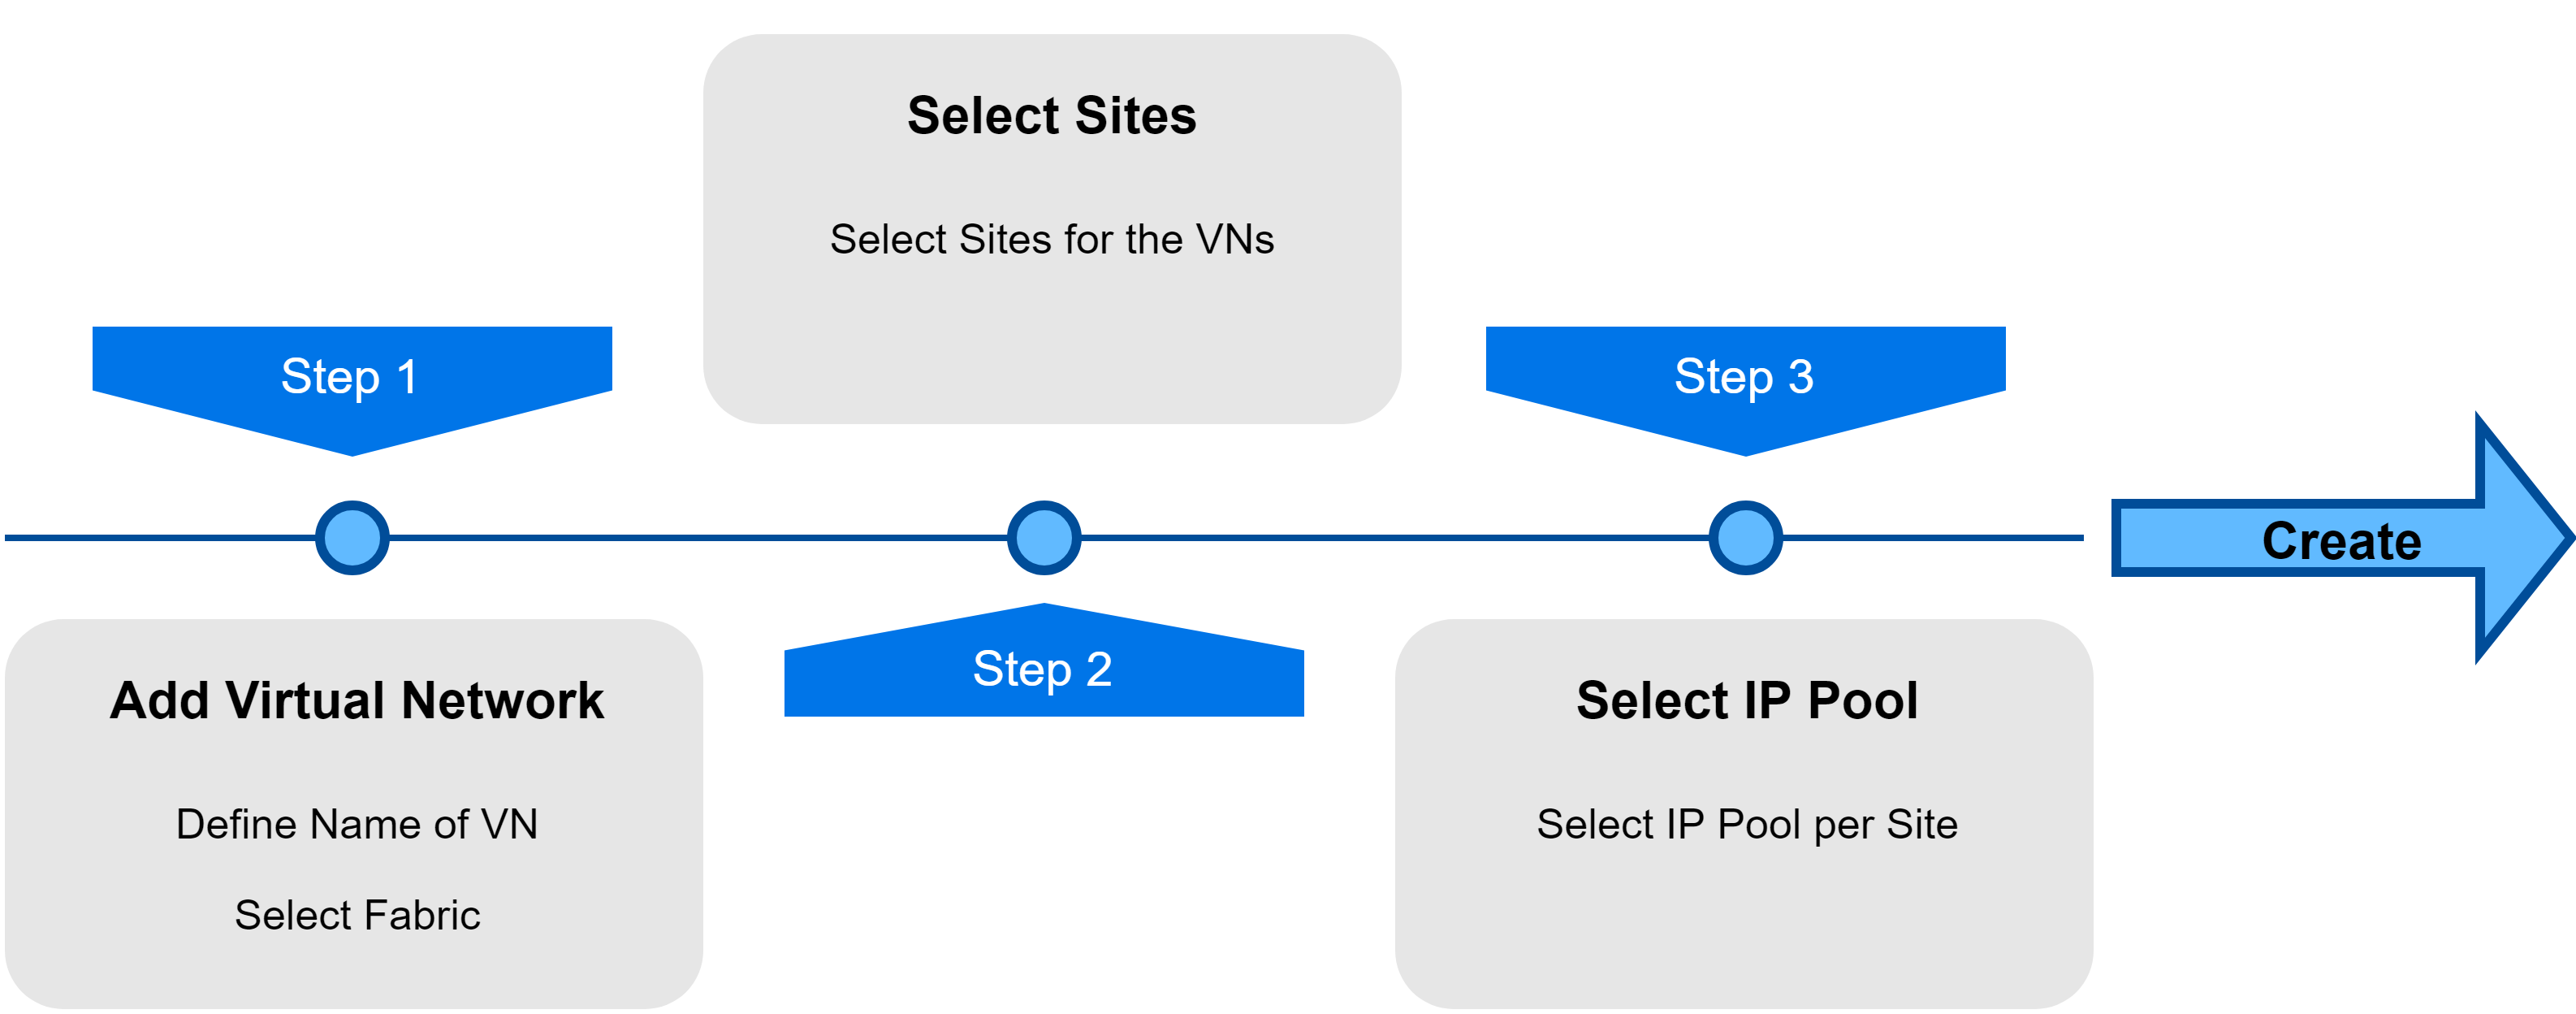
\includegraphics[width=0.8\linewidth]{img/Abstrahierung/addvirtualnetwork}
	\caption{Add Virtual Network}
	\label{fig:Add Virtual Network}
\end{figure}

Um den Wizard zu starten, kann im Orchestrationtool im Home \textit{Virtual Networks $\rightarrow$ Add Virtual Networks} ausgewählt werden. So startet der Wizard mit den in der Abbildung (siehe Abbildung \ref{fig:Add Virtual Network}: Add Virtual Network) aufgezeigten Schritten und man kann Schritt für Schritt die gewünschten Informationen angeben.

Der Wizard verwendet die APIs des DNA Centers, sowie der Netzwerkgeräte. Beim DNA Center mussten teilweise undokumentierte API Endpoints verwendet werden, da die nötigen Funktionen ansonsten nicht verfügbar sind. Dies birgt das Risiko, dass sich diese in Zukunft ändern und die Applikation angepasst werden muss.

\subsubsection{Virtual Machine Management}

Das Virtual Machine Management zeigt alle virtuallen Maschinen auf NFVIS an. Des Weiteren wird der aktuelle Status der VMs, sowie die Netzwerkinterfaces angezeigt. Zudem ist es möglich, eine VM über das Web Interface zu starten oder zu stoppen.

\begin{figure}[H]
	\centering
	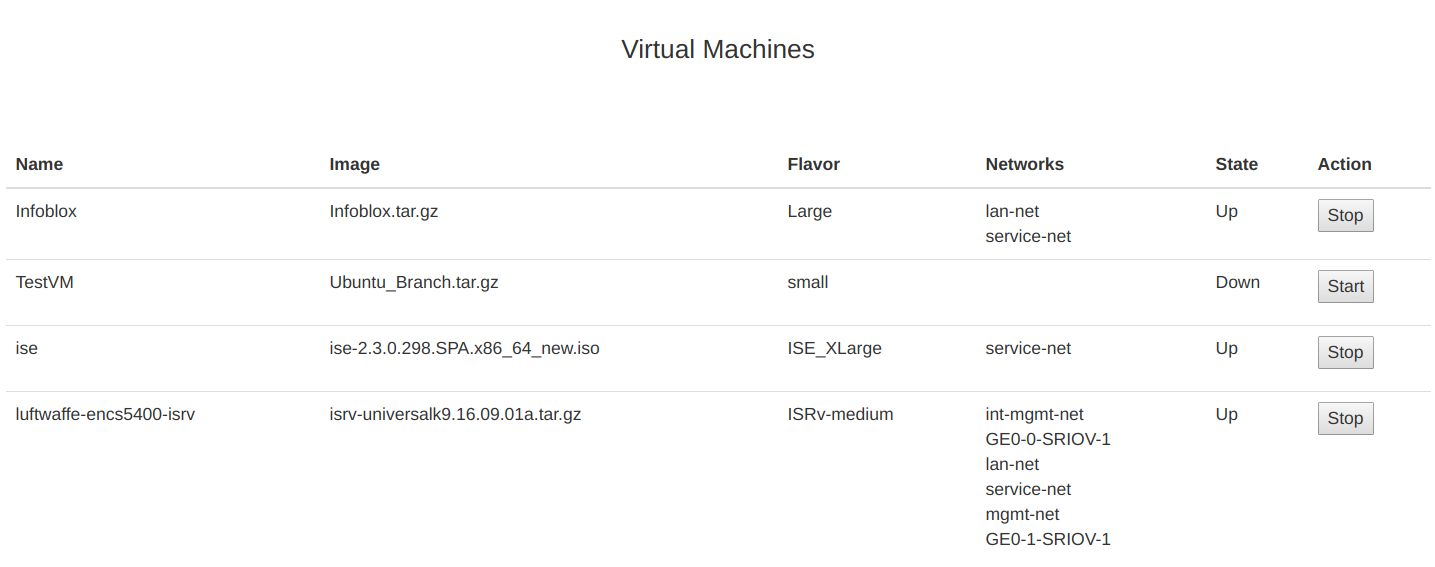
\includegraphics[width=0.8\linewidth]{img/Abstrahierung/vm-management.png}
	\caption{VM Management}
	\label{fig:VM Management}
\end{figure}

\subsubsection{Configuration History}

Dieser Use Case konnte nicht mehr vollständig umgesetzt werden. Derzeit kann nur die aktuelle Konfiguration angezeigt werden. Die Anzeige einer History ist noch nicht implementiert.

\begin{figure}[H]
	\centering
	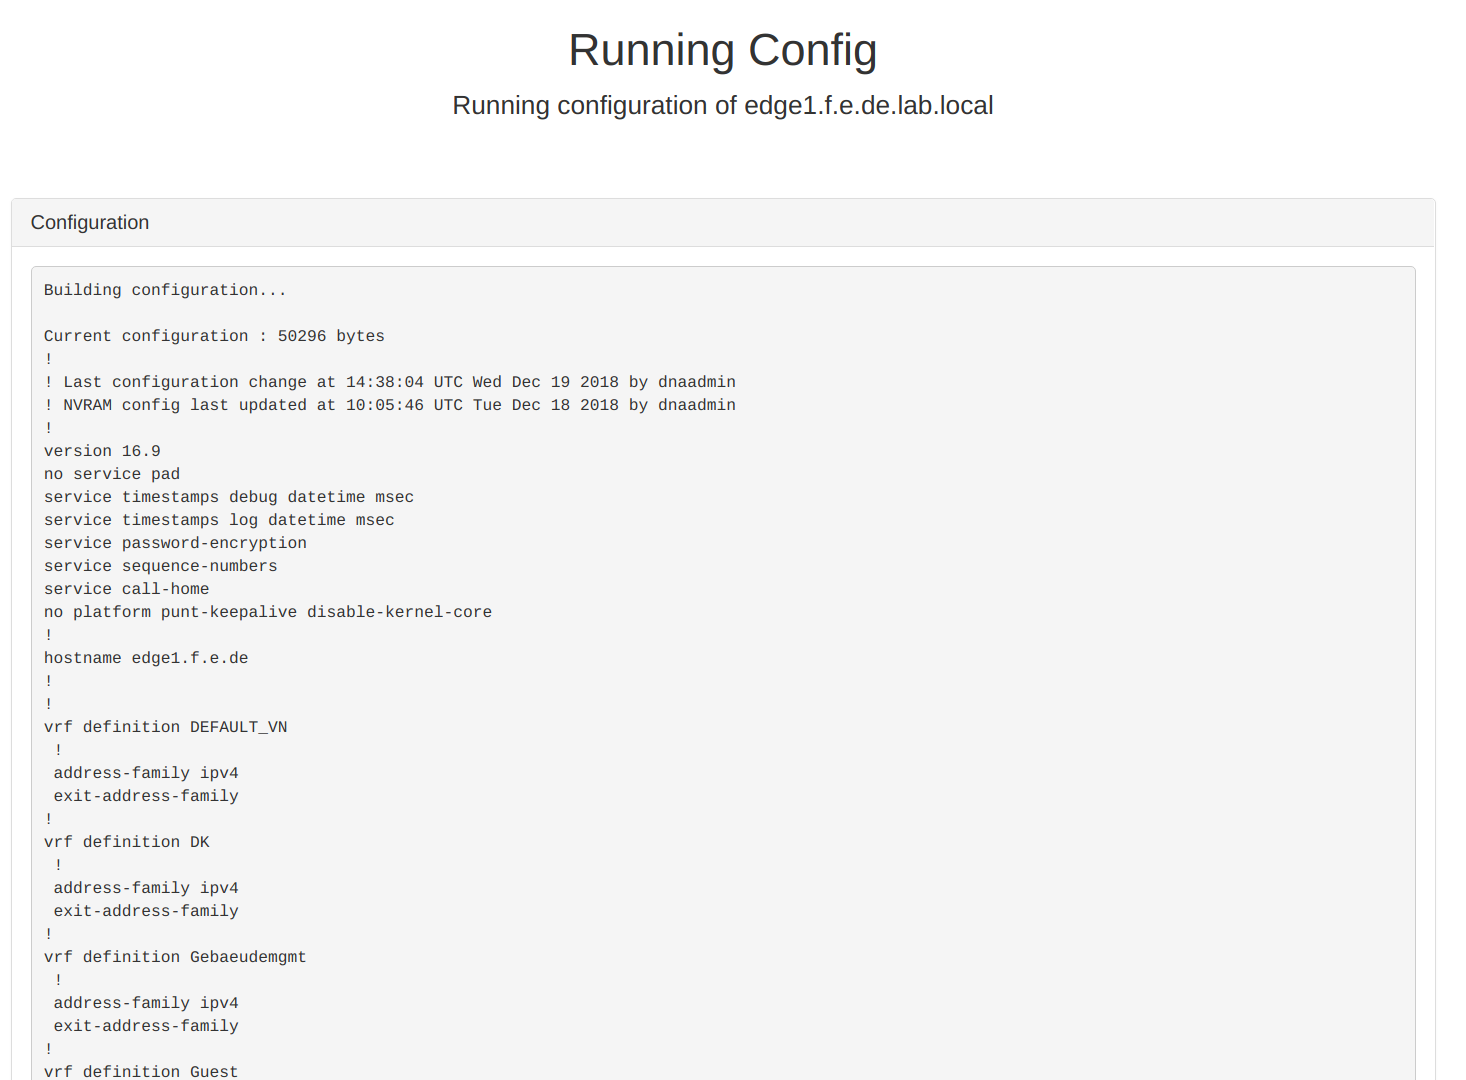
\includegraphics[width=0.8\linewidth]{img/Abstrahierung/running-config.png}
	\caption{Running Config}
	\label{fig:Running Config}
\end{figure}







\section{Feature Requests und Bugs}
Im Folgenden werden Feature Requests und Bugs aufgeführt, die während dieser Arbeit aufgetreten sind. Diese wurden mittesl "Make a Wish" Funktion des DNA Centers an Cisco gemeldet. Alle erwähnten Punkte beziehen sich auf das DNA Center in Version 1.2.5.


\newcommand{\bugreport}[9]{
\subsection{#1}
	\begin{table}[H]
		\rowcolors{2}{gray!25}{white}
		\centering
		\begin{tabularx}{\textwidth}{| l | X |}
			\hline
			Komponente   & #2       \\
			\hline
			Priorität   & #3       \\
			\hline
			Beschreibung   & #4  \\ 
			\hline
			Konsequenzen   & #5  \\ 
			\hline
			Workaround & #6 \\
			\hline
			Reproduzieren & #7	\\
			\hline
			Reporter  & #8 \\
			\hline
			Feedback Cisco & #9 \\
			\hline
		\end{tabularx}
		\caption{Bug: #1}
	\end{table}
}

\newcommand{\featureRequest}[5]{
	\subsection{#1}
	\begin{table}[H]
		\rowcolors{2}{gray!25}{white}
		\centering
		\begin{tabularx}{\textwidth}{| l | X |}
			\hline
			Komponente   & #2       \\
			\hline
			Beschreibung   & #3  \\ 
			\hline
			Reporter  & #4 \\
			\hline
			Feedback Cisco & #5 \\
			\hline
		\end{tabularx}
		\caption{Feature Request: #1}
	\end{table}
}

\featureRequest
% Titel
{Template Zuweisung}
% Komponente
{\textit{Design $\rightarrow$ Network Profiles}}
% Beschreibung
{Templates können nur Gerätetypen (z.Bsp. Switches oder Router) zugewiesen werden. Es wäre wünschenswert, wenn diese auch verschiedenen Rollen zugewiesen werden könnten. Beispielsweise allen Border Nodes.
}
% Reporter
{Sandro Kaspar}
% Feedback Cisco
{}

\featureRequest
% Titel
{Template Versionierung}
% Komponente
{\textit{Template Editor $\rightarrow$ Create Template}}
% Beschreibung
{Templates können versioniert werden. Allerdings lassen sich ältere Versionen nur anschauen. Folgende Funktionen wären hilfreich:
\begin{itemize}
	\item Restore alter Templateversionen
	\item Diffs zwischen verschiedenen Versionen anzeigen
\end{itemize}
}
% Reporter
{Sandro Kaspar}
% Feedback Cisco
{}

\bugreport
% Titel
{Upload Image}
% Komponente
{\textit{Design $\rightarrow$ Image Repository $\rightarrow$ Import}}
% Dringlichkeit
{Mittel}
% Beschreibung
{Nach dem Uploaden eines Images, wird dieses nicht im WebGui angezeigt. Erst nach mehreren Minuten erscheint das zuvor hochgeladene Image.
}
% Konsequenzen
{Der User geht davon aus, dass der Upload fehlgeschlagen ist und versucht dies erneut.}
% Workaround
{Keiner}
%Reproduzieren
{
	\begin{enumerate}
		\item \textit{Design $\rightarrow$ Image Repository $\rightarrow$ Import}
		\item File auswählen
		\item Warten bis der Upload abgeschlossen ist
		\item Image wird nicht angezeigt
		\subitem Nach mehreren Minuten erscheint das Image
	\end{enumerate}
}
% Reporter
{Sandro Kaspar}
% Feedback Cisco
{}


\bugreport
% Titel
{Claim Device}
% Komponente
{\textit{Provision $\rightarrow$ Inventory}}
% Dringlichkeit
{Niedrig}
% Beschreibung
{Nach dem Hinzufügen oder Claimen eines Devices werden verschiedene Informationen als "null" angezeigt. Hier sollten die korrekten Informationen oder falls noch nicht verfügbar einfach nichts angezeigt werden.
}
% Konsequenzen
{Unschönes UI}
% Workaround
{Keiner}
%Reproduzieren
{
	\begin{enumerate}
		\item \textit{Provision $\rightarrow$ Inventory $\rightarrow$ Unclaimed Devices $\rightarrow$ Claim Device}
	\end{enumerate}
}
% Reporter
{Sandro Kaspar}
% Feedback Cisco
{}

\bugreport
% Titel
{Image Checksum}
% Komponente
{\textit{Design $\rightarrow$ Image Repository}}
% Dringlichkeit
{Mittel}
% Beschreibung
{Wird auf ein Image geklickt, sodass die Detailinformationen angezeigt werden, wird die Checksumme vom "Make a Wish" Button überdeckt. Dies tritt bei FullHD Auflösung oder kleiner auf.
}
% Konsequenzen
{Checksumme nicht lesbar}
% Workaround
{Grössere Auflösung}
%Reproduzieren
{
	\begin{enumerate}
		\item \textit{Design $\rightarrow$ Image Repository $\rightarrow$ Auf Image klicken}
	\end{enumerate}
}
% Reporter
{Sandro Kaspar}
% Feedback Cisco
{}


\bugreport
% Titel
{Provision Status "Failed"}
% Komponente
{\textit{ Provision $\rightarrow$ Devices $\rightarrow$ Inventory}}
% Dringlichkeit
{Niedrig}
% Beschreibung
{Der Provision Status wird als "Failed" angezeigt, auch wenn die Provisionierung funktioniert hat. Dies wird zur Zeit auf ewig so angezeigt, sollte im Verlauf irgendwann einmal etwas fehlgeschlagen sein. Dazu kommt, dass wenn man auf See Details klickt, die Einträge mit Success angezeigt werden. Zuerst muss also herausgefunden werden, bei welchem Workflow dies aufgetreten ist. Mit erneutem Klick auf See Details auf dem Workflow, werden die einzelnen Schritte des Workflows angezeigt.
}
% Konsequenzen
{Verwirrung das Problem vorhanden, obwohl keines besteht}
% Workaround
{Keiner}
%Reproduzieren
{
	
}
% Reporter
{Jessica Kalberer}
% Feedback Cisco
{}


\bugreport
% Titel
{Provision Template Status Failed}
% Komponente
{\textit{ Provision $\rightarrow$ Devices $\rightarrow$ Inventory}}
% Dringlichkeit
{Niedrig}
% Beschreibung
{Der Status des Schrittes im Workflow des Provisioning wird als Failed angezeigt, weil der Name schon gesetzt wurde. Es wird die Meldung "Template IOS Banner Template:2 is already deployed with same params,. Not deploying it." angezeigt. Der Name wurde zwar schon einmal mit dem Template deployed, jedoch handelte es sich nicht um den gleichen.
}
% Konsequenzen
{Verwirrung das Problem vorhanden, obwohl keines besteht}
% Workaround
{Keiner}
%Reproduzieren
{
	\begin{enumerate}
		\item \textit{Provision $\rightarrow$ Devices $\rightarrow$ Inventory}
		\item Gewünschtes Device auswählen
		\item \textit{Actions $\rightarrow$ Provision}
		\item Template für Namensänderung wählen
		\item \textit{Provision}
	\end{enumerate}
}
% Reporter
{Jessica Kalberer}
% Feedback Cisco
{}

\bugreport
% Titel
{Fabric Custom View}
% Komponente
{\textit{ Provision $\rightarrow$ Fabric $\rightarrow$ Layout}}
% Dringlichkeit
{Mittel}
% Beschreibung
{Wenn eine Custom View erstellt wird und diese ausgewählt wird, werden die Devices nicht mehr als Teil der Fabric angezeigt. 
}
% Konsequenzen
{Fabric lässt sich in der Custom View nicht bearbeiten}
% Workaround
{Keiner}
%Reproduzieren
{
	\begin{enumerate}
		\item \textit{Provision $\rightarrow$ Fabric $\rightarrow$ Layout}
		\item Custom View erstellen
		\item Custom View anzeigen
	\end{enumerate}
}
% Reporter
{Sandro Kaspar}
% Feedback Cisco
{}

\bugreport
% Titel
{Fabric Default View}
% Komponente
{\textit{ Provision $\rightarrow$ Fabric $\rightarrow$ Layout}}
% Dringlichkeit
{Niedrig}
% Beschreibung
{Wenn eine Custom View erstellt wird und anschliessend als Default View definiert wird, hat dies keinen Einfluss auf die Default View. Es wird weiterhin die Default View von Cisco angezeigt
}
% Konsequenzen
{Custom Views sind nutzlos, wenn jedes Mal die gewünschte View gewählt werden muss.}
% Workaround
{Keiner}
%Reproduzieren
{
	\begin{enumerate}
		\item \textit{Provision $\rightarrow$ Fabric $\rightarrow$ Layout}
		\item Custom View erstellen
		\item Custom View als Default setzen
		\item Reload
	\end{enumerate}
}
% Reporter
{Sandro Kaspar}
% Feedback Cisco
{}
%\section {Testprotokolle}


%\section{Umsetzung}




%\section{Vorgehen} \label{versuch1}

\section{Ergebnisdiskussion}


\subsection{Zielsetzungen}


\subsection{Bugs}





\section{Schlussfolgerungen}

\subsection{Erreichte Ziele}
Wie in den Ergebnissen erwähnt, konnten die gesetzten Ziele der Bachelorarbeit fast vollständig erreicht werden. 
 
 
\subsection{Mögliche Verbesserungen}
Die in dieser Arbeit bisher aufgetretenen Bugs können sicherlich Verbessert werden. Auch wäre es schön, wenn das DNA Center eine Wegweisung, durch zum Beispiel einen Wizard, durch die komplexen Abläufe bereitstellen würde. Dies kann jedoch nun auch durch Verwendung der API und entwicklung eines eigenen Orchestrierungstool etwas umgangen und für sich vereinfacht werden.


Das eigene Orchestrierungstool kann aber auf jeden Fall noch endlos erweitert werden. Dabei können nicht nur verschiedene Abläufe durch einen Wizard vereinfacht werden, welche zur Zeit im DNA Center sehr viel manuellen Aufwand benötigen, sondern auch weitere Eigenentwicklungen implementiert werden.


 \subsection{Zukunft}
Seit vielen Jahren betreiben viele Unternehmen ihre Netzwerke gleich, manuell mit Konsolenkabeln, Telnet, SHH, CLI oder anderen Tools. In der Zeit der Digitalisierung wird es immer schwieriger solch grosse Netze kosteneffizient zu Warten. Vor fast zwei Jahren hat sich Cisco zum Ziel gesetzt das Netzwerk neu zu erfinden und dabei das DNA Center entwickelt. Im Frühling 2018 hat Cisco das DNA Assurance eingeführt, um das Monitoring des gesamten Netzwerkes enorm zu vereinfachen. Im Sommer 2018 hat Cisco nun das DNA Center für Entwickler zugänglich gemacht. Dank der neuen offenen DNA Center Platform können nun über die APIs eigene Anwendungen entwickelt werden.\\

Cisco hat das DNA Center innerhalb der letzten Jahren immer weiterentwickelt und viele vorher vorhandene Bugs behoben. Bleibt nur zu hoffen, dass sich dies so weiterentwickelt. \\

Doch nicht nur Cisco, sondern auch andere Konkurrenten fördern die Automatisierung des Netzwerkes, um Unternehmensweite Netzwerke bereitzustellen. Dabei setzen sie ebenfalls auf eine zentrale Plattform, mit welcher das Monitoring und Provisioning ausserordentlich vereinfacht wird.

\section{Abkürzungsverzeichnis}
\begin{acronym}[SEPSEPSEP]
	\acro{AAA}{Authentication, Authorization, and Accounting}
	\acro{ACL}{Access Control List}
	\acro{AP}{Access Point}
	\acro{API}{Application Programming Interface}
	\acro{ARP}{Address Resolution Protocol}
	\acro{BGP}{Border Gateway Protocol}
	\acro{CCO}{Cisco Connection On-line}
	\acro{CIMC}{Cisco Integrated Management Controller}
	\acro{CLI}{Command-Line Interface}
	\acro{CMD}{Cisco Meta Data}
	\acro{CP}{Control Plane}
	\acro{CVD}{Cisco Validated Design}
	\acro{C3850}{Catalyst 3850}
	\acro{C9300}{Catalyst 9300}
	\acro{DHCP}{Dynamic Host Configuration Protocol}
	\acro{DNA}{Cisco Digital Network Architecture}
	\acro{DNS}{Domain Name System}
	\acro{dot1x}{IEEE 802.1X Standard zur Authentifizierung}
	\acro{ECNS}{Enterprise Network Compute System}
	\acro{EID}{Endpoint Identifier}
	\acro{ETR}{Egress Tunnel Router}
	\acro{FE}{Fabric Edge}
	\acro{FUB}{Führungsunterstützungsbasis}
	\acro{GW}{Gateway}
	\acro{HTDB}{Host Tracking Database}
	\acro{IEEE}{Institute of Electrical and Electronics Engineers}
	\acro{IGP}{Interior Gateway Protocol}
	\acro{IOS}{Internetworking Operating System}
	\acro{IP}{Internet Protocol}
	\acro{IPAM}{IP-Adress-Management}
	\acro{ISE}{Cisco Identity Services Engine}
	\acro{IS-IS}{Intermediate System to Intermediate System}
	\acro{ISR}{Integrated Service Routers}
	\acro{ITR}{Ingress Tunnel Router}
	\acro{KVM}{Kernel-based Virtual Machine}
	\acro{LAN}{Local Area Network}
	\acro{LISP}{Locator/ID Separation Protocol}
	\acro{MnT}{Monitoring and Troubleshooting Node}
	\acro{MS}{Map Server}
	\acro{MSMR}{Map Server/Map Resolver}
	\acro{MR}{Map Resolver}
	\acro{NTP}{Network Time Protocol}
	\acro{NFV}{Network Functions Virtualization}
	\acro{NFVIS}{NFV Infrastructure Software}
	\acro{PAN}{Policy Administration Node}
	\acro{PETR}{Proxy Egress Tunnel Router}
	\acro{PITR}{Proxy Ingress Tunnel Router}
	\acro{PnP}{Plug and Play}
	\acro{PSN}{Policy Service Node}
	\acro{PXG}{PxGrid}
	\acro{pxGrid}{Platform Exchange Grid}
	\acro{qcow}{QEMU Copy On Write}
	\acro{RADIUS}{Remote Authentication Dial-In User Service}
	\acro{REST}{Representational State Transfer}
	\acro{RLOC}{Routing locator}
	\acro{SDA}{Software-Defined Access}
	\acro{SDK}{Software Development Kit }
	\acro{SDN}{Software-Defined Networking}
	\acro{SGACL}{Scalable Group Access Control List}
	\acro{SGT}{Security Group Tags}
	\acro{SNMP}{Simple Network Management Protocol}
	\acro{STP}{Spanning Tree Protocol}
	\acro{SXP}{Security Group Tag Exchange Protocol}
	\acro{TFTP}{Trivial File Transfer Protocol}
	\acro{TTL}{Time To Live}
	\acro{UDP}{User Datagram Protocol}
	\acro{URL}{Uniform Resource Locator}
	\acro{VLAN}{Virtual Local Area Network}
	\acro{VM}{Virtual Machine}
	\acro{VN}{Virtual Network}
	\acro{VNI}{Virtual Extensible LAN Network Identifier}
	\acro{VPN}{Virtual Private Network}
	\acro{VRF}{Virtual Routing and Forwarding}
	\acro{VSS}{Virtual Switching Systems}
	\acro{VTEP}{Virtual Extensible LAN Tunnel Endpoint}
	\acro{VXLAN}{Virtual Extensible LAN}
	\acro{VXLAN-GPO}{Virtual Extensible LAN Group Policy Option}
	\acro{WAN}{Wide Area Network}
	\acro{Web}{World Wide Web}
	\acro{WLAN}{Wireless Local Area Network}
	\acro{WLC}{Wireless LAN Controller}
	\acro{WSGI}{Web Server Gateway Interface}
	\acro{XML}{Extensible Markup Language}
	\acro{xTR}{x Tunnel Router}
\end{acronym}




\newpage
\appendix
\pagenumbering{Roman}

%\section{Installationsanleitung}


%\section{Benutzerhandbuch}


\section{Projektmanagement}

\subsection{Projektübersicht}
Das Hauptziel dieser Bachelorarbeit...

\subsubsection{Ziele der Projektes}


\subsection{Projektorganisation}
Diese Bachelorarbeit wird von zwei Personen umgesetzt und durch zwei Betreuer überwacht.

\subsubsection{Organisationsstruktur}


\subsection{Management Abläufe}
Für die Umsetzung der Bachelorarbeit stehen insgesamt 14 Wochen und pro Person 360 Stunden zur Verfügung. In einer Woche liegt das Arbeitspensum von 26 Stunden pro Person vor. Das Projekt startet am 17. September 2018 und endet am 21. Dezember 2018.

\subsubsection{Zeitliche Planung}
Die zeitliche Planung, sowie die Verwaltung der Arbeitspakete erfolgte auf Waffle.io. Die Planung wird während dem Projekt laufend aktualisiert und angepasst. Die Arbeitszeiten werden während der Arbeitsausführung mit Toggle erfasst.



\subsubsection{Meilensteine}
Folgende Meilensteine sind für das Projekt definiert:



\subsubsection{Arbeitspakete}
Alle Arbeitspakete werden in Waffle.io erfasst und sind unter folgendem Link ersichtlich:
\href{Waffle.io}{https://waffle.io/night28/HSR\_BA}
\subsubsection{Besprechungen}
Die Besprechungen mit dem Betreuer finden an den nachfolgend aufgelisteten Tagen statt:
\begin{itemize}
	\item jeden Mittwoch zwischen 10.30 - 11.30 Uhr
\end{itemize}

Offene Traktanden und Probleme werden mit dem Betreuer diskutiert. Nach dieser Besprechung wird jeweils in einem Team-Meeting das weitere Vorgehen geplant.


\subsection{Infrastruktur}
Die Organisation der Arbeit und Teammitglieder wird durch folgende Werkzeuge unterstützt:

\begin{figure}[H]
	\centering
	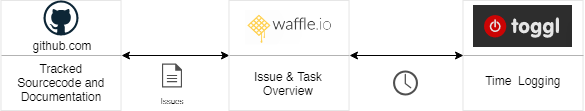
\includegraphics[width=13cm]{img/EingesetzteToolsZurOrganisation.png}
	\caption{Übersicht über die Verknüpfung der eingesetzten Werkzeuge zur internen Organisation.}
	\label{fig:Interne Organisationsstruktur}
\end{figure} 

Unsere Tools sind unter folgenden Links einsehbar:
\paragraph{GitHub} \href{https://github.com/night28/HSR\_BA}{https://github.com/night28/HSR\_BA} 

\paragraph{Waffle.io} \href{https://waffle.io/night28/HSR\_BA}{https://waffle.io/night28/HSR\_BA}

\paragraph{Toggl} \href{https://toggl.com/}{https://toggl.com/}
 
\subsection{Risiko Management}

\subsubsection{Umgang mit Risiken}


\subsubsection{Risiken}


\subsubsection{Eingetretene Risiken}

\section{Zeitmanagement}

\subsection{Zeitaufwand pro Person und Kategorie}


\subsection{Verteilung pro Kategorie}


\subsection{Zeitaufwand pro Woche}

%\section{Bugs}

\section{Persönliche Summaries}

\subsection{Sandro Kaspar}

Ich war sehr erfreut, dass wir eine Folgearbeit für unsere Studienarbeit machen durften. Insbesondere weil ich mich schon immer sehr stark für Netzwerktechnologien interessiert habe. Mit dieser Arbeit wurde mir zudem die Möglichkeit geboten, mit sehr aktuellen Technologien und Produkten zu arbeiten, die ich aus dem Arbeitsalltag noch nicht kenne. Des Weiteren ist die Aufgabenstellung auf Grund der Grösse und Struktur des Industriepartners sehr herausfordernd.\\
Da das DNA Center in der Studienarbeit noch sehr neu war, freute ich mich darauf, zu sehen wie sich dieses weiterentwickelt hat, was verbessert wurde und welche neuen Funktionen hinzugekommen sind. Ebenfalls sehr spannend war der Einsatz des ENCS 5400, ein Produkt, das ich in dieser Form zuvor noch nicht kannte. 
Erfreulicherweise kann ich sagen, dass sich das DNA Center sehr stark verbessert hat. Die Softwarequalität hat stark zugenommen und es wurden neue Features hinzugefügt, welche die Arbeit mit dem DNA Center erleichtern. An den eingesetzten Produkten, dem DNA Center, der ISE und dem ENCS 5400 gibt es sicherlich immer noch viel Verbesserungspotenzial, besoners was die Softwarequalität und die intuitive Bedienung der Produkte anbelangt. Wenn diese aber wie bisher stetig weiterentwickelt werden, bin ich zuversichtlich, dass sich diese Technologien durchsetzen werden.\\
Die Arbeit im Team funktionierte meiner Meinung nach sehr gut. Ebenfalls sehr gut gestaltete sich die Zusammenarbeit mit unseren Betreuern, Experten und dem Industriepartner. \\
Abschliessend kann ich sagen, dass ich während dieser Arbeit sehr viel gelernt habe und meine Fähigkeiten weiterentwickeln konnte. Es war spannend mit modernsten Produkten und zukunftsweisenden Technologien zu arbeiten und zu sehen wie sich diese bewähren.

\subsection{Jessica Kalberer}

% !TeX encoding = UTF-8
\section{Sitzungsprotokolle}

\subsection{Sitzungsprotokoll 18.09.2018}

\paragraph{Sitzungsteilnehmer}
\begin{itemize}	
	\item Laurent Metzger 
	\item Urs Baumann 
	\item Patrick Mosimann
	\item Sandro Kaspar
	\item Jessica Kalberer
\end{itemize}

\paragraph{Traktanden}
\begin{itemize}
	\item Besprechung genaue Aufgabenstellung und nächste Schritte
	\item Chat für BA
	\item Traktanden vor Meetings Liste an Betreuer? 
	\item ISE Lizenzen abgelaufen
\end{itemize}

\paragraph{Beschlüsse (Diskussion)}
\begin{itemize}	
	\item Heute Kickoff Besprechung für die Bachelorarbeit
	\item Wie krisenresistent ist das Software Defined Netzwerk?
	\item FUB hat folgende Anforderungen und Aufteilung der Bachelorarbeit vorgesehen:
	\begin{itemize}
		\item 10\% der Bachelorarbeit Analyse, wo kritische Stellen der Lösung sind
		\begin{itemize}
			\item Begrenzungen allgemein
			\item DNAC muss keine Internetverbindung haben, da kein Lizenzenforcement bestehen
			\item Wireless Controler erwähnen, dass diese redundant sein müssen, aber in nachfolgender Arbeit eher ausklammern.
			\item Router mit virtuellen Maschinen (berücksichtigen für kritische Stellen, beispielsweise für Spiegelung von Radix Server)
		\end{itemize}
		\item 45\% Analysieren wo die Lösung aufgrund der kritischen Stellen verbessert werden kann
		\begin{itemize}
			\item Transit Fabric oder VRF-Lite vergleichen, was ist besser einzusetzen?
			\item Design anpassen aufgrund der Änderungen
			\item ziemlich sicher hierachisches Modell, da mehrere Fabrics für FUB nötig
			\item für die ganze Planung werden wahrscheinlich Docker Container verwendet
		\end{itemize}
		\item 45\% Implementation mit einem Business Controller (einem abstrahierten Modell)
		\begin{itemize}
			\item 3-4 Use Cases, welche wir von der FUB erhalten
			\item API Controller verwenden: Ziel der Automatisierung, damit nur noch MAC angegeben werden muss und nicht in WebGUI etliche Einstellungen vorgenommen werden können
		\end{itemize}
	\end{itemize}
	\item Patrick wird uns bei Neuerungen informieren, welche von den Releases her für die Umsetzung der Bachelorarbeit relevant sind.
	\item Zielsetzung vorläufig für 24. September 2018: ein laufendes DNA Center, mit allen Geräten sauber provisioned. Darum wird Patrick vor der wöchentlichen Sitzung mit uns zusammensitzen.
	\item Detaillierte Aufgabenstellung wird noch geschrieben, von Cisco und FUB reviewt und uns nächste Woche übergeben	
	\item Traktanden jeweils wieder im Voraus an Betreuen senden
\end{itemize}

\paragraph{Offene Punkte (erledigt vor nächster Sitzung)} \mbox{}
\begin{table}[H]
	\rowcolors{2}{gray!25}{white}
	\centering
	\begin{tabularx}{\textwidth}{X | p{4.5cm}}
		\rowcolor{gray!50}
		\textbf{Was} & \textbf{Verantwortlichkeit} \\
		\hline	
		DNAC Cleanup mit Patrick	& Sandro, Jessica \\	
	\end{tabularx}
	\label{tab:my-label}
\end{table}

\paragraph{Nächster Termin}
\begin{itemize}	
	\item Meeting mit Patrick: 19. September 2018, 09.00 Uhr
	\item Wöchentliches Meeting: 19. September 2018, 10.30 Uhr, 60 Minuten (ausgefallen)
\end{itemize}

\paragraph{Kommende Abwesenheiten} \mbox{}\\
keine

\newpage





\subsection{Sitzungsprotokoll 26.09.2018}

\paragraph{Sitzungsteilnehmer}
\begin{itemize}	
	\item Laurent Metzger 
	\item Urs Baumann 
	\item Patrick Mosimann
	\item Sandro Kaspar
	\item Jessica Kalberer
\end{itemize}

\paragraph{Traktanden}
\begin{itemize}	
	\item Aktueller Stand 
	\begin{itemize}
		\item Anpassungen Architektur
		\item LAN-Automation erfolgreich
		\item Updates der Switches laufend
		\item Fabric noch ausstehend
	\end{itemize}
	\item Aufgabenstellung	
\end{itemize}

\paragraph{Beschlüsse (Diskussion)}
\begin{itemize}	
	\item Saubere Fabric mit Standort Jona fertigstellen
	\item Erster Teil der BA Starten: Analyse
	\begin{itemize}
		\item NTP beachten, was passiert wenn dieser Dienst verlegt wird
	\end{itemize}
	\item Zweiter Teil: Phase Absicherung (bis Ende Oktober erledigt)
	\item Detailbeschreibungen der drei Phasen in Aufgabenstellung ersichtlich. Diese bekommen wir noch im laufe des heutigen Tages.
\end{itemize}

\paragraph{Offene Punkte (erledigt vor nächster Sitzung)} \mbox{}
\begin{table}[H]
	\rowcolors{2}{gray!25}{white}
	\centering
	\begin{tabularx}{\textwidth}{X | p{4.5cm}}
		\rowcolor{gray!50}
		\textbf{Was} & \textbf{Verantwortlichkeit} \\
		\hline	
		Fabric Jona abschliessen & Sandro \& Jessica \\
		Projektplan anhand Aufgabenstellung erarbeiten & Sandro \& Jessica \\
		Teil 1: Analyse Phase starten & Sandro \& Jessica \\
	\end{tabularx}
	\label{tab:my-label}
\end{table}

\paragraph{Nächster Termin}
\begin{itemize}	
	\item Wöchentliches Meeting: 03. Oktober 2018, 10.30 Uhr, 60 Minuten
\end{itemize}

\paragraph{Kommende Abwesenheiten} \mbox{}\\
keine

\newpage





\subsection{Sitzungsprotokoll 03.10.2018}

\paragraph{Sitzungsteilnehmer}
\begin{itemize}	
	\item Laurent Metzger 
	\item Urs Baumann (abwesend)
	\item Patrick Mosimann (abwesend)
	\item Sandro Kaspar
	\item Jessica Kalberer
\end{itemize}

\paragraph{Traktanden}
\begin{itemize}	
	\item Analyse besprechen
	\item VN für Backups ausstehend
	\item Projektplanung
\end{itemize}

\paragraph{Beschlüsse (Diskussion)}
\begin{itemize}	
	\item Analyse und Traktanden werden für Review per Slack an Betreuer gesendet (Terminkonflikt)
\end{itemize}

\paragraph{Offene Punkte (erledigt vor nächster Sitzung)} \mbox{}
\begin{table}[H]
	\rowcolors{2}{gray!25}{white}
	\centering
	\begin{tabularx}{\textwidth}{X | p{4.5cm}}
		\rowcolor{gray!50}
		\textbf{Was} & \textbf{Verantwortlichkeit} \\
		\hline	
		Analyse überarbeiten & Jessica \& Sandro  \\
	\end{tabularx}
	\label{tab:my-label}
\end{table}

\paragraph{Nächster Termin}
\begin{itemize}	
	\item Wöchentliches Meeting: 10. Oktober 2018, 10.30 Uhr, 60 Minuten
\end{itemize}

\paragraph{Kommende Abwesenheiten} \mbox{}\\
keine

\newpage





\subsection{Sitzungsprotokoll 10.10.2018}

\paragraph{Sitzungsteilnehmer}
\begin{itemize}	
	\item Laurent Metzger 
	\item Urs Baumann
	\item Patrick Mosimann
	\item Sandro Kaspar
	\item Jessica Kalberer
\end{itemize}

\paragraph{Traktanden}
\begin{itemize}	
	\item Liefertermin von ENCS 5000
	\item Besprechung der Analyse
	\item Freischaltung Images ISR 4430 und ENCS 5000 (Service Contract Required)
\end{itemize}

\paragraph{Beschlüsse (Diskussion)}
\begin{itemize}
	\item Analyse Besprechnung
	\begin{itemize}
		\item SDA Architektur und Design
		\begin{itemize}
			\item Informationen mit neustem Release 1.2.5 updaten
			\item Maximum Scale - nur 20 Fabric Domains? Es gibt mehr Kantone!
		\end{itemize}
		\item Cisco Severity and Escalation Guidelines implementieren
		\begin{itemize}
			\item Eigene Severity erstellen (Beispielsweise ist in den Cisco Guidelines der DNA Ausfall erst bei Severity 3) 
			\item Verfügbarkeiten mit Severity ergänzen
		\end{itemize}
		\item Verfügbarkeiten
		\begin{itemize}
			\item LISP Map Server / Control Plane Node
			\begin{itemize}
				\item LISP abhängig von der Platzierung (ENCS Control Plane virtualisieren, gibt es Möglichkeiten?), Phyton Script das eventuell Map Cache statisch konfiguriert
				\item Severity 1
				\item dezentrale Lösung wenn möglich
			\end{itemize}
			\item ISE / Radius
			\begin{itemize}
				\item Was passiert mit schon bestehenden angemeldeten Personen bei Ausfall?
				\item Annahmen treffen und diese in nächsten Teilen der Arbeit testen
				\item Severity 1
				\item dezentrale Lösung
			\end{itemize}
			\item SGT Access List
			\begin{itemize}
				\item Detaillierter beschreiben was in welchen Fällen passiert
				\item Beispiel:  SGT Access Listen werden nur auf Control Node gespeichert (nur wegen SXP)
				\item Beispiel: sobald Client weg ist, wird dieser wieder aus der SGT Access List gelöscht? Was passiert bei nächster Anmeldung? 
				\item Severity 1
				\item dezentrale Lösung möglich?
			\end{itemize}
			\item Border Node
			\begin{itemize}
				\item Das meiste sollte funktionieren, solange lokaler ISE/Radius etc. vorhanden
				\item keine dezentrale Lösung nötig
				\item Wie funktioniert die Redundanz?
				\item Wie ist die Konvergenz (ISIS/BGP)? Gibt es eine Optimierung?
				\item 
			\end{itemize}
			\item Fusion Router
			\begin{itemize}
				\item Kein Leaking zwischen VRFs?
				\item Herr Metzger kennt sich mit dieser Materie sehr gut aus. Nicht zu viel Zeit verlieren und direkt mit ihm die Konfiguration anschauen.
				\item Urs kann bei Fragen beim Orchestration Tool konsultiert werden.
				\item dezentrale Lösung
			\end{itemize}
			\item DHCP, NTP, DNS
			\begin{itemize}
				\item DNS UND NTP können mehrere angegeben werden, so das im Notfall einfach der andere Server genommen wird
				\item Severity 2
			\end{itemize}
			\item Lizenzen
			\begin{itemize}
				\item Severity 4 - falls diese aber enforced werden wird es Severity 1 oder Severity 2
			\end{itemize}
		\end{itemize}
	\end{itemize}
	\item Projektmanagement
	\begin{itemize}
		\item Risiken gut, aber im Bild sind R5 und R6 nicht ersichtlich
	\end{itemize}
	\item Liefertermin von ENCS 5000 wird noch abgeklärt
	\item nächste Schritte
	\begin{itemize}
		\item Verbindungen mit VRF-Lite und Transit Fabric (VXLAN)
		\item VRF Route Leaking einrichten (da sonst keine Kontrolle wenn alles in einer Routing Tabelle)
		\item anpassung Architektur - Router als zweiter Legacy einrichten
		\item Bei FUB ist die Telefonie zentral - sie müssen keine IP Connectivität haben
	\end{itemize}
	\item Dokument wieder an Herrn Metzger und Urs senden, damit sie Reviewen können
\end{itemize}


\paragraph{Offene Punkte (erledigt vor nächster Sitzung)} \mbox{}
\begin{table}[H]
	\rowcolors{2}{gray!25}{white}
	\centering
	\begin{tabularx}{\textwidth}{X | p{4.5cm}}
		\rowcolor{gray!50}
		\textbf{Was} & \textbf{Verantwortlichkeit} \\
		\hline	
		Analyse überarbeiten & Jessica \& Sandro  \\
		Dokument für Review an Betreuer senden & Jessica \\
		Teil 2: Absicherung vorbereiten & Jessica \& Sandro \\
	\end{tabularx}
	\label{tab:my-label}
\end{table}

\paragraph{Nächster Termin}
\begin{itemize}	
	\item Wöchentliches Meeting: 17. Oktober 2018, 10.30 Uhr, 60 Minuten
\end{itemize}

\paragraph{Kommende Abwesenheiten} \mbox{}\\
keine

\newpage





\subsection{Sitzungsprotokoll 17.10.2018}

\paragraph{Sitzungsteilnehmer}
\begin{itemize}	
	\item Laurent Metzger 
	\item Urs Baumann
	\item Sandro Kaspar
\end{itemize}

\paragraph{Traktanden}
\begin{itemize}	
	\item Liefertermin ENCS 5000
	\item Besprechung aktueller Stand
	\item Nächste Schritte
\end{itemize}

\paragraph{Beschlüsse (Diskussion)}
\begin{itemize}	
	\item Analyse grösstenteils abgeschlossen
	\item Liefertermin für ENCS 5000 war für Mitte November vorgesehen, wird aber beschleunigt
	\item nächste Schritte
	\begin{itemize}
		\item zweiten Router in Betrieb nehmen
		\item Devices updaten
		\item Transit Fabric einrichten
		\item vrf Route Leaking
		\item Absicherungen aus Analyse erarbeiten
	\end{itemize}
	\item Teil 3 kann auch parallel zu Teil 2 begonnen werden
	\item Nächste Woche findet keine Sitzung statt
	\item Review des Dokuments per PDF
\end{itemize}

\paragraph{Offene Punkte (erledigt vor nächster Sitzung)} \mbox{}
\begin{table}[H]
	\rowcolors{2}{gray!25}{white}
	\centering
	\begin{tabularx}{\textwidth}{X | p{4.5cm}}
		\rowcolor{gray!50}
		\textbf{Was} & \textbf{Verantwortlichkeit} \\
		\hline	
		 Zweiten Router in Betrieb nehmen & Jessica \& Sandro \\
		 Devices updaten & Jessica \& Sandro \\
		 Transit Fabric einrichten & Jessica \& Sandro  \\
		 VRF Route Leaking & Jessica \& Sandro \\
		 Teil2: Absicherung erarbeiten (beginnen) & Jessica \& Sandro \\
	\end{tabularx}
	\label{tab:my-label}
\end{table}

\paragraph{Nächster Termin}
\begin{itemize}	
	\item Wöchentliches Meeting: 31. Oktober 2018, 10.30 Uhr, 60 Minuten
\end{itemize}

\paragraph{Kommende Abwesenheiten} \mbox{}\\
keine

\newpage



\subsection{Sitzungsprotokoll 07.11.2018}

\paragraph{Sitzungsteilnehmer}
\begin{itemize}	
	\item Urs Baumann
	\item Sandro Kaspar
	\item Jessica Kalberer
\end{itemize}

\paragraph{Traktanden}
\begin{itemize}	
	\item Bewertungsraster der Studienarbeit
	\item Liefertermin ENCS 5000 (KW46)
	\item Feedback Analyse
	\item Besprechung aktueller Stand Absicherung
	\begin{itemize}
		\item ISE / Radius Absicherung Vorschläge?
		\item SGT ACL Absicherung Vorschläge?
		\item DHCP
	\end{itemize}
	\item Nächste Schritte
	\item Zwischenpräsentation 
	\begin{itemize}
		\item Wünsche und Anregungen für Inhalt
		\item Termin möglichst spät im November
	\end{itemize}
	\item Endtermin BA - wird abgeklärt
	\item Use Cases für Teil 3 ausstehend
\end{itemize}

\paragraph{Beschlüsse (Diskussion)}
\begin{itemize}	
	\item ISE Cluster (3 Nodes) - keine autonome Standorte
	\item DNAC lässt nur einen Radius Eintrag zu - Loadbalancer
	\item DHCP Infoblox Active / Active Setup oder Active / Passiv mit Backup Pool - Variante A und B definieren
	\item Verlängerung Endtermin BA
	\item ENCS 5000
	\begin{itemize}
		\item NTP
		\item DHCP Backup
		\item Subinterfaces
	\end{itemize}
	\item Zwischenpräsentation
	\begin{itemize}
		\item Design Ansätze
		\item Aktueller Stand
	\end{itemize}
	\item Offene Traktanden an unseren Betreuer senden
	\item Zusätzliche Module für beide ISR für ein Full-Mesh Setup bei FUB anfragen
\end{itemize}

\paragraph{Offene Punkte (erledigt vor nächster Sitzung)} \mbox{}
\begin{table}[H]
	\rowcolors{2}{gray!25}{white}
	\centering
	\begin{tabularx}{\textwidth}{X | p{4.5cm}}
		\rowcolor{gray!50}
		\textbf{Was} & \textbf{Verantwortlichkeit} \\
		\hline	
		Zweiten Router in Betrieb nehmen & Jessica \& Sandro \\
		Transit Fabric einrichten & Jessica \& Sandro  \\
		VRF Route Leaking & Jessica \& Sandro \\
		Teil2: Absicherung abschliessen / umsetzen & Jessica \& Sandro \\
	\end{tabularx}
	\label{tab:my-label}
\end{table}

\paragraph{Nächster Termin}
\begin{itemize}	
	\item Wöchentliches Meeting: 14. November 2018, 10.30 Uhr, 60 Minuten
\end{itemize}

\paragraph{Kommende Abwesenheiten} \mbox{}\\
keine




\newpage




\subsection{Sitzungsprotokoll 14.11.2018}

\paragraph{Sitzungsteilnehmer}
\begin{itemize}	
	\item Laurent Metzger
	\item Urs Baumann
	\item Patrick Mosimann
	\item Sandro Kaspar
	\item Jessica Kalberer
\end{itemize}

\paragraph{Traktanden}
\begin{itemize}	
	\item Bewertungsraster der Studienarbeit
	\item Liefertermin ENCS 5000 (KW46)
	\item Feedback Analyse noch ausstehend
	\item Besprechung Absicherung
	\begin{itemize}
		\item ISE / Radius Absicherung Vorschläge?
		\item SGT ACL Absicherung Vorschläge?
	\end{itemize}
	\item Nächste Schritte
	\item Zwischenpräsentation 
	\begin{itemize}
		\item Wünsche und Anregungen für Inhalt
	\end{itemize}
	\item Endtermin BA
	\item Use Cases für Teil 3 ausstehend
\end{itemize}

\paragraph{Beschlüsse (Diskussion)}
\begin{itemize}	
	\item Erweiterte Module für ISR4431 erhalten, schon eingebaut und alles verkabelt
	\item ENCS 5000 noch ausstehend
	\item BA Endtermin formell noch ausstehend, aber wahrscheinlich bis Mitte Januar verlängert	
	\item ISE / Radius Absicherung ähnlich wie DHCP
	\item SGT ACL Absicherung - sinnvolle Replizierung?
	\begin{itemize}
		\item bleiben nach Timeout nur zwei Minuten auf Gerät
		\item Beispiel1: lokal auf 9300 SGACLs alle fünf Minuten sichern und diese bei Ausfall wieder eintragen. Nachteil: Host-Mobility funktioniert nicht, aber lokal kann weitergearbeitet werden.
		\item Beispiel2: global komplett alle SGACLs auf alle Geräte verteilen. Vorteil: Alle Geräten haben jederzeit alle Einträge. Nachteil: Die Maximum Scale Recommendations der SGACLs sind pro Gerät anders. C3850 - 1500 SGACLs, C9300 
		\item TrustSec SXP Speaker/Listener auf C3850 und C9300 definieren
		\item 3850 als Gateway  für 9300 Listener definieren
	\end{itemize}
	\item Aktuellstes Dokument bis Donnerstagabend an Betreuer senden, Feedback erfolgt nächste Woche
	\item Bewertungsraster der Studienarbeit erhalten wir noch, damit eventuelle Verbesserungen noch in Zwischenpräsentation einfliessen können
	\item Use Cases werden von unseren Betreuern festgelegt
	\begin{itemize}
		\item Use Case 0 aus Aufgabenstellung: wenn zwei VRFs zusammen kommunizieren, werden die Fabric und der Fusion Router gleichzeitig konfiguriert.
	\end{itemize}
\end{itemize}

\paragraph{Offene Punkte (erledigt vor nächster Sitzung)} \mbox{}
\begin{table}[H]
	\rowcolors{2}{gray!25}{white}
	\centering
	\begin{tabularx}{\textwidth}{X | p{4.5cm}}
		\rowcolor{gray!50}
		\textbf{Was} & \textbf{Verantwortlichkeit} \\
		\hline	
		Transit Fabric einrichten & Jessica \& Sandro  \\
		VRF Route Leaking & Jessica \& Sandro \\
		Teil2: Absicherung abschliessen / umsetzen & Jessica \& Sandro \\
		Dokument an Betreuer senden & Jessica \\
	\end{tabularx}
	\label{tab:my-label}
\end{table}

\paragraph{Nächster Termin}
\begin{itemize}	
	\item Wöchentliches Meeting: 21. November 2018, 10.30 Uhr, 60 Minuten
\end{itemize}

\paragraph{Kommende Abwesenheiten} \mbox{}\\
keine



\newpage





\subsection{Sitzungsprotokoll 21.11.2018}

\paragraph{Sitzungsteilnehmer}
\begin{itemize}	
	\item Laurent Metzger
	\item Jessica Kalberer
\end{itemize}

\paragraph{Traktanden}
\begin{itemize}	
	\item Bewertungsraster der Studienarbeit
	\item  5400 Übergabe
	\item Feedback Analyse
	\item Feedback Absicherung
	\item Zwischenpräsentation 
	\begin{itemize}
		\item Wünsche und Anregungen für Inhalt
		\item Dauer
	\end{itemize}
	\item Use Cases für Teil 3
	\begin{itemize}
		\item Vorschlag: Config-History mit divs
	\end{itemize}
\end{itemize}

\paragraph{Beschlüsse (Diskussion)}
\begin{itemize}	
	\item ENCS 5400 erhalten und wird diese Woche in Betrieb genommen
	\item Besprechung wird wegen Terminkonflikten auf Donnerstag den 22.11.2018 verschoben
\end{itemize}

\paragraph{Offene Punkte (erledigt vor nächster Sitzung)} \mbox{}
\begin{table}[H]
	\rowcolors{2}{gray!25}{white}
	\centering
	\begin{tabularx}{\textwidth}{X | p{4.5cm}}
		\rowcolor{gray!50}
		\textbf{Was} & \textbf{Verantwortlichkeit} \\
		\hline
		ENCS in Betrieb nehmen & Jessica \& Sandro \\	
		Transit Fabric einrichten & Jessica \& Sandro  \\
		VRF Route Leaking & Jessica \& Sandro \\
		Teil2: Absicherung abschliessen / umsetzen & Jessica \& Sandro \\
	\end{tabularx}
	\label{tab:my-label}
\end{table}

\paragraph{Nächster Termin}
\begin{itemize}	
	\item Wöchentliches Meeting: 22. November 208
\end{itemize}

\paragraph{Kommende Abwesenheiten} \mbox{}\\
keine


\newpage






\subsection{Sitzungsprotokoll 22.11.2018}

\paragraph{Sitzungsteilnehmer}
\begin{itemize}	
	\item Laurent Metzger
	\item Urs Baumann
	\item Patrick Mosimann
	\item Sandro Kaspar
	\item Jessica Kalberer
\end{itemize}

\paragraph{Traktanden}
\begin{itemize}	
	\item Bewertungsraster der Studienarbeit
	\item Feedback Analyse
	\item Feedback Absicherung
	\item Zwischenpräsentation 
	\begin{itemize}
		\item Wünsche und Anregungen für Inhalt
		\item Dauer
	\end{itemize}
	\item Use Cases für Teil 3
	\begin{itemize}
		\item Vorschlag: Config-History mit divs
	\end{itemize}
\end{itemize}

\paragraph{Beschlüsse (Diskussion)}
\begin{itemize}	
	\item Zwischenpräsentation
	\begin{itemize}
		\item Dauer 20-30 Minuten
		\item Theorie zum Anfang mit kritischen Komponenten
		\item Überblick
		\item Aktueller Stand
		\item Absicherung kurz, nicht zu detailliert
		\item Demo 
		\begin{itemize}
			\item Border Ausfall Video mit LISP Map Cache
			\item Registrierung von Client über LISP 
			\item Ping Verluste aufzeichnen und begründen
		\end{itemize}
		\item Diskussion wie wichtig Infoblox ist
		\item Use Cases für Phase 3 besprechen
	\end{itemize}	
	\item MSMR testen - Map Cache Ausfall simulieren (evtl. in Präsentation vorstellen)
	\item Radius - Maximale Instanzen dokumentieren. ISE Radius und Freeradius genauer untersuchen, ob sie das selbe Protokoll z.B. tacacs+ benutzen. Routing Kosten hinterlegen, damit der Pfad zum ISE priorisiert wird und ansonsten den eigenen Freeradius in seiner Fabric nimmt. Anycast über IS-IS. Underlay oder Overlay?
	\item DHCP Backup Pool mit komplett anderem Range
	\item Use Cases für Teil 3
	\begin{itemize}
		\item Archdrive für Config-History mit divs (Zeitstempel, Passwörter und weiteres überschreiben)
	\end{itemize}
	\item Besprechung vor Zwischenpräsentation, für kurzen Einblick
	\item Bewertungsraster der Studienarbeit und Feedback der Dokumentation erhalten wir per Slack
\end{itemize}

\paragraph{Offene Punkte (erledigt vor nächster Sitzung)} \mbox{}
\begin{table}[H]
	\rowcolors{2}{gray!25}{white}
	\centering
	\begin{tabularx}{\textwidth}{X | p{4.5cm}}
		\rowcolor{gray!50}
		\textbf{Was} & \textbf{Verantwortlichkeit} \\
		\hline	
		Teil2: Absicherung abschliessen / umsetzen & Jessica \& Sandro \\
		Zwischenpräsentation vorbereiten & Jessica \& Sandro \\
	\end{tabularx}
	\label{tab:my-label}
\end{table}

\paragraph{Nächster Termin}
\begin{itemize}	
	\item Vorbesprechung Zwischenpräsentation: 26. November 2018, 60 Minuten
	\item Zwischenpräsentation: 28. November 2018, 10.30 Uhr, 60 Minuten
\end{itemize}

\paragraph{Kommende Abwesenheiten} \mbox{}\\
keine







\includepdf[scale=0.9,pages={1},pagecommand=\section{Erklärungen}\subsection{Eigenständigkeitserklärung}]{pdfincludes/eigenstaendigkeit}
\newpage

\includepdf[scale=1.0,pages={1},pagecommand=\subsection{Urheberrechtsvereinbarung}]{pdfincludes/urheberrecht}

\renewcommand{\listtablename}{Tabellenverzeichnis}
\listoftables
\addcontentsline{toc}{section}{\listtablename}
\renewcommand{\listfigurename}{Abbildungsverzeichnis}
\listoffigures
\addcontentsline{toc}{section}{\listfigurename}
\clearpage
\renewcommand{\refname}{Literaturverzeichnis}
\addcontentsline{toc}{section}{Literaturverzeichnis}
\begin{thebibliography}{}

	\bibitem{sda-designguide-aug2018} SDA Design Guide \textit{Software-Defined Access Design Guide August}, 2018 (URL: \url{https://www.cisco.com/c/dam/en/us/td/docs/solutions/CVD/Campus/CVD-Software-Defined-Access-Design-Guide-2018AUG.pdf}), 02.10.2018
	
	\bibitem{sda-designguide-sept2018} SDA Design Guide \textit{Software-Defined Access Design Guide September}, 2018 (URL: \url{https://www.cisco.com/c/dam/en/us/td/docs/solutions/CVD/Campus/CVD-Software-Defined-Access-Design-Sol1dot2-2018SEP.pdf})
		
	\bibitem{cisco-severity-guidelines} Severity Guidelines \textit{Cisco Severity and Escalation Guidelines}, 2018 (URL: \url{https://www.cisco.com/c/dam/en_us/about/doing_business/legal/service_descriptions/docs/Cisco_Severity_and_Escalation_Guidelines.pdf}), 11.10.2018
	
	\bibitem{LISP-mobility} LISP Host Mobility Solution \textit{LISP Host Mobility Solution}, 2018 (URL: \url{https://www.cisco.com/c/en/us/td/docs/solutions/Enterprise/Data_Center/DCI/5-0/LISPmobility/DCI_LISP_Host_Mobility/LISPmobile_3.html}), 17.10.2018
	
	\bibitem{LISP-impact} LISP Impact \textit{Locator/ID Separation Protocol (LISP) Impact}, 2016, (URL: \url{https://tools.ietf.org/html/rfc7834}), 31.10.2018
	
	\bibitem{sda-deploymentguide-oct2018} SDA Deployment Guide  \textit{SDA Deployment Guide Oktober}, 2018, (URL: \url{https://www.cisco.com/c/dam/en/us/td/docs/solutions/CVD/Campus/CVD-Software-Defined-Access-Deployment-Guide-Sol1dot2-2018OCT.pdf}), 07.11.2018
	
	\bibitem{sda-segmentation-may2018} SDA Segmentation Design Guide \textit{SDA Segmentation Design Guide May}, 2018 (URL: \url{https://www.cisco.com/c/dam/en/us/td/docs/solutions/CVD/Campus/CVD-Software-Defined-Access-Segmentation-Design-Guide-2018MAY.pdf}), 15.11.2018

	\bibitem{dnac-cluster} Cisco Digital Network Architecture Center Installation Guide \textit{Release 1.2}, 2018 (URL: \url{https://www.cisco.com/c/en/us/td/docs/cloud-systems-management/network-automation-and-management/dna-center/1-2/install/b_dnac_install_1_2/b_dnac_install_1_2_chapter_0101.html}), 08.12.2018
	
	\bibitem{ise-scale} Cisco Identity Services Engine Installation Guide \textit{Network Deployments in Cisco ISE}, 2018 (URL: \url{https://www.cisco.com/c/en/us/td/docs/security/ise/2-4/install_guide/b_ise_InstallationGuide24/b_ise_InstallationGuide24_chapter_00.html}), 10.12.2018
\end{thebibliography}




\end{document}

